%=========================================================================
% (c) Michal Bidlo, Bohuslav Křena, Jaroslav Dytrych 2015


%===============================================
% Introduction
%===============================================
\chapter*{Introduction}
\addcontentsline{toc}{chapter}{Introduction}
A recommender system is a computer program that is able to predict the~preference of~a~user for~a~certain item. It can do so by looking at past behaviours of users, meaning the history of their interactions with other items. These interactions can be represented differently in~various systems. Some systems enable users to rate items and express their preference explicitly, e.g. in the form of a star rating~on~a~scale from~1~to~10. Other systems may not have the ability to allow their users to give explicit feedback and~hence have to determine the significance of interactions on~their own, considering not only the preference a~user gives to~a~certain item, but also the confidence the system has in~this information.


All things considered, these systems can create a truly powerful tool and~it~is~no~surprise they found their way to a wide area of application. Shopping centres track recent purchases of their customers and create customized offers for them. Internet televisions recommend shows and movies similar to those users already watched and liked. E-shops can display products users are more likely to buy above the others. Behind all these applications, there is a recommender system. They help companies maximize their sales and~improve user experience, enable users to find things they are interested~in faster and easier. Moreover, their relevance is~still getting stronger as the~internet is~becoming more personalized and~their performance is still improving with collecting larger amounts of~data along with higher processing capabilities.

The main purpose of this thesis was to create a system recommending web articles in~the~domain \texttt{developers.redhat.com}. The objective was to implement an architecture based on a probabilistic model that had not been used for this task before and evaluate its performance by comparing it with other models created using conventional methods.

Chapter \ref{datasets} compares known dataset types and their different ways of representing feedback from users. It also describes the dataset, that this thesis is working with. Chapter \ref{approaches} aims to explain the most popular approaches used to build recommender systems and describe their advantages and weaknesses. Chapter \ref{proposed} presents the proposed architecture, that is based on the Skip-gram negative sampling model originally used in the Word2Vec method to create word embeddings. The proposed architecture applies this model to the recommendation problem. Finally, chapter \ref{implementation} discusses the most important implementation details of all created models. And chapter \ref{evaluation} explains the process of their evaluation, compares the models with state-of-the-art and reviews the obtained results. All the created models can be found on the enclosed DVD and also in a repository created on GitHub \footnote{GitHub repository: \url{https://github.com/JanKoci/Recommender-systems}}.


%===============================================
% The Recommendation Problem
%===============================================
\chapter{The Recommendation Problem} \label{rec_problem}

The formal definition of a recommendation problem can be described as suggested in~\cite{Toward}:
Let $C$ be the set of all users and $S$ the set of all items in a dataset. Let $u$ be the utility function that measures the usefulness of item $s$ for user $c$. The usefulness measure can be a real positive number and is assigned to every user-item pair. We can express this idea as a mapping of~the~cartesian product of sets $C$ and $S$ to a set of values $R$: 
$$u: \, C \times S \rightarrow R$$

This mapping is surjective, meaning two different elements from $C \times S$ can be mapped to the same value from $R$. The goal of recommendation is then to find a set of items that would maximize the utility function for a user: 
\begin{equation}
    \forall c \in C: \quad S'_{c} = \argmax_{s \in \mathcal{S}} u(c, s)
\end{equation}
Where $c$ is a user from the set $C$, $s$ is an item from the set $S$, $u$ is the utility function and $S'_{c}$ is a set of items that maximize the utility function for user $c$.
The utility of a user-item pair is often represented as a rating the user gave the item. That leads us to the central problem of recommender systems. The utility function is not defined on the whole $C \times S$ space, but only on the items previously rated by the users. Consequently, the utility function has to be approximated to the whole $C \times S$ space. 
%%%%%%%%% Is it good ??? %%%%%%%%%%%%%%
The problem can be divided into two parts. The~first part is to define the utility function to measure the known user-item interactions. The~second part is to estimate the unknown interactions, usually by building a probabilistic model on the set of known user-item interactions. Finally, when the unknown ratings are estimated, the system can recommend items with the highest predicted ratings.
%%%%%%%%%%%%%%%%%%%%%%%%%%%%%%%%%%%%%%%

These procedures, however, are hard to define as they can differ on every system. The~measures of usefulness or importance can sometimes be application specific. \\ News websites give a much bigger weight to recently published articles than to something that happened three years ago, because its users want to know, what happened lately. Whereas users of~an~internet television would not mind watching a movie from the ’90s. 


%===============================================
% Datasets
%===============================================
\chapter{Datasets for Recommender Systems} \label{datasets}

In order to be able to make recommendations, the system needs data. As it~was already mentioned in section \ref{rec_problem}, the system works with a set of users and a set of items. A typical dataset then consists of interactions between these users and items. Such interactions, however, can have a different meaning on every system, giving the recommender specific feedback about the behaviour of its users. Based on the representation of this feedback, datasets are classified into explicit feedback and implicit feedback datasets. 

In the \texttt{explicit} feedback datasets, interactions reflect the preferences of users very accurately. They are created as users give items a specific rating, e.g. on a scale from 1 to 10, telling the system how much they liked them. The \texttt{implicit} feedback datasets are harder to deal with. In these systems, users do not explicitly rate items. Instead, the system has to guess their preferences, given by~certain clues. These clues can be for example: how many times the user clicked on~an~article, how many times did the user watch a~show, or what keywords did the user search for.
Similarly, as~in~any~other machine learning system, the~amount of~data, as~well~as its quality, is~crucial. The~more information the~system gets, the~better it should perform.

Datasets can be stored e.g. in~a~CSV file, where each row represents one interaction, that consists of unique user and item identifiers and a numeric value, that describes the interaction e.g.~a~rating.


%===============================================
% Explicit
%===============================================
\section{Explicit Feedback Datasets}

Explicit feedback datasets reflect the preferences of users very accurately, as users explicitly tell the system, how much they like certain items, usually by giving them a rating. They further enable the existence of negative feedback. That means they allow their users not only to express what items they like but also what items they dislike. Hence the interactions between users and items that the system is interested in are created every time a rating is given. These interactions are often stored in a so-called interaction matrix, in which every row represents a unique user and every column a unique item. \pagebreak

\begin{table}[h!]
    \centering
    \begin{tabular}{@{}cccc@{}}
    \toprule
          & Seven & The Shining & Pretty Woman \\ \midrule
    \rowcolor[HTML]{EFEFEF}
    Julia & 2.5   &             & 5.0          \\
    Jack  &       & 5.0         & 1.5          \\
    \rowcolor[HTML]{EFEFEF}
    Brad  & 5.0   &             &              \\ \bottomrule
    \end{tabular}
    \caption{Simple example of an interaction matrix. It contains users in rows and items, or movies in this particular example, in columns. Values in this matrix represent the rating users gave the movies. That means user Brad rated the movie Seven with 5 stars etc. Empty fields indicate users have not rated the movie yet.}
    \label{table:Interaction_matrix}
\end{table}

The interaction matrix, as can be seen in table \ref{table:Interaction_matrix}, can be very sparse. That means it contains a~lot of zero values, where no interaction has occurred. These fields contain a~special value, one that does not appear in the rating scale, usually a zero. In most datasets, this sparsity can reach over 90\%, meaning 90\% of the values are zeros. 
Therefore these matrices are often stored in a memory efficient data structure, where only the non-zero values are stored, together with their position in the original matrix. Then, assuming the sparsity is 90\%, instead of having one matrix of size $100K \times 100K$, we have 3 matrices of~size $1K \times 1$. The first matrix contains all non-zero values and the other two matrices contain indexes of~rows and~columns in the original matrix.


One example of~existing public explicit feedback datasets could be the \texttt{Movielens} \footnote{Dataset was retrieved from \url{https://grouplens.org/datasets/movielens/}} dataset. In this dataset users rate movies by giving them a~certain number of~stars, from half~a~star being the~worst rating, to 5 stars being the~best. This dataset is available in several forms varying in size from 100K interactions up to 20M, as shown in~table \ref{table:movielens}. \\

\begin{table}[h!]
    \centering
    \begin{tabular}{@{}ccccc@{}}
    \toprule
    \textbf{Size} & \textbf{Number of users} & \textbf{Number of movies} & \textbf{Sparsity} & \textbf{Released} \\ \midrule
    \rowcolor[HTML]{EFEFEF}
    20M           & 138 000                                          & 27 000                                            & 99.5\%            & 10/2016           \\
    10M           & 72 000                                           & 10 000                                            & 98.6\%            & 1/2009            \\
    \rowcolor[HTML]{EFEFEF}
    1M            & 6 000                                            & 4 000                                             & 95.8\%            & 2/2003            \\
    100K          & 600                                              & 9 000                                             & 98.1\%            & 9/2018            \\ \bottomrule
    \end{tabular}
    \caption{This table gives a brief review of available Movielens data sets and their content.}
    \label{table:movielens}
\end{table}

Some systems use a different approach, where ratings are given to items in form of~thumbs up or down. This type of binary rating tells the system only whether the user does or does not like the~item. It tells nothing about the~quantity, how much they like it. This type of ratings is used in platforms by companies like Netflix, Inc. or YouTube, LLC. Some of them converted to this design from using star ratings, as it appeared to be more beneficial. 

One of~them is referred to as per-user bias. Users often interpret the~rating scale differently. A~3-star rating could indicate a~greater preference for a~user whose average given rating is, as~supposed, 2.5 stars. However, if a~user only gives big ratings around 4 or~5 stars, his 3-star rating would be interpreted as not~so~significant. One other problem that Netflix ran into, was that users tended to give old movies a~big rating, not because they personally liked it, but because they are generally considered to~be good. This resulted in recommending rather an~old movie than something new that the user would much rather watch.

%===============================================
% Implicit
%===============================================
\section{Implicit Feedback Datasets} \label{implicit_datasets}
The explicit feedback is clearly very convenient for the~system and~results in~more~accurate recommendations. However, this kind of~feedback is~not~always available. Some applications simply do~not have the~ability to~allow their users to~rate every single item they interact~with. Like shopping centres, that track the purchases of their customers. Most of~them would probably not really enjoy rating how satisfied they were with~the~butter they bought yesterday. This is when the~implicit feedback comes in useful.

The implicit feedback is~not obtained directly from~users, but by~observing their~behaviour and~interactions with~items. The interactions here, instead of explicit ratings, are the actions of users, like visiting a webpage or buying a product. The numeric value representing an interaction can then be e.g. how many times did a user visit a certain webpage, how much time did he spend on it etc. It is important to~identify the~unique features of~implicit feedback compared to the~explicit, as mentioned in paper \cite{Implicit}:
\begin{enumerate}
    \item There is no negative feedback. In explicit datasets, users could give an item a low rating to tell the system, they do not like it. Implicit feedback does not have this~ability. By observing the behaviour of users, the system can only assume, what items they probably like. Also, it cannot assume that not interacting with an~item is an~indication of not liking it. The user may not even know this item exists.

    \item The feedback is very noisy. That means, there is a lot of misinformation. Sometimes users may click on an article by mistake, or may not like it at all after reading it.
    
    \item In explicit datasets, the numeric value of interaction represents preference. As~stated in the previous point, implicit datasets are very noisy. Therefore an interaction between a user and an item cannot directly imply he prefers the item, it only tells the~system that he might like it. And so rather than preference, here the numeric value of interaction represents confidence. The more a~user interacts with a~certain item, the~more confident the~system is about his preference for this item.
\end{enumerate}
Authors of paper \cite{Implicit} suggest a new method for working with this confidence. Let $r_{ui}$ be the numeric value of interaction between a user $u$ and an item $i$. This value can represent e.g. how many times the user visited this page or how much time did he spend on it. Then, the~authors introduce a new variable $p_{ui}$, that is a binary representation of the $r_{ui}$ value:
\begin{equation} \label{eq:implicit_preference}
p_{ui} = 
\begin{cases}
    1, & r_{ui} > 0 \\
    0, & r_{ui} = 0
\end{cases}
\end{equation}
The $p_{ui}$ value indicates, that the user could have a preference for this item. More important, however, is how confident the system is about this preference. The confidence value is closely associated with the $r_{ui}$ value. As the $r_{ui}$ value grows, the system has a stronger indication that the user indeed likes the item and the confidence value increases. The confidence, that the system has in the interaction between a user $u$ and an item $i$, can be computed using the following formula as suggested in paper \cite{Implicit}:
\begin{equation} \label{eq:lin_conf}
c_{ui} = 1 + \alpha r_{ui}
\end{equation}
Where $\alpha > 0$ is a constant that controls the rate of increase. Another potential formula for confidence, used when the range of $r_{ui}$ values is wide, uses logarithm:
\begin{equation} \label{eq:log_conf}
c_{ui} = 1 + \alpha \log(1 + r_{ui} / \epsilon)
\end{equation}
Where $\alpha>0$ and $\epsilon>0$ are both parameters of the model. This method is especially useful to eliminate the big values of $r_{ui}$, which could be caused by an accident. If the system measured the time spent on a webpage, an extremely big $r_{ui}$ value could occur, for example, when a user left his computer to go to the toilet.

Implicit datasets are definitely harder to deal with. They contain much less useful information, are harder to obtain and the systems are harder to evaluate. Despite all the difficulties, they are used very frequently across the internet, as for some systems it is not possible to allow users to rate their items. In some cases it is not even likeable. Users simply do not want to waste their time giving any feedback. Therefore they still keep their relevance and are also the topic of this thesis. 

\begin{figure}[H]
    \centering
    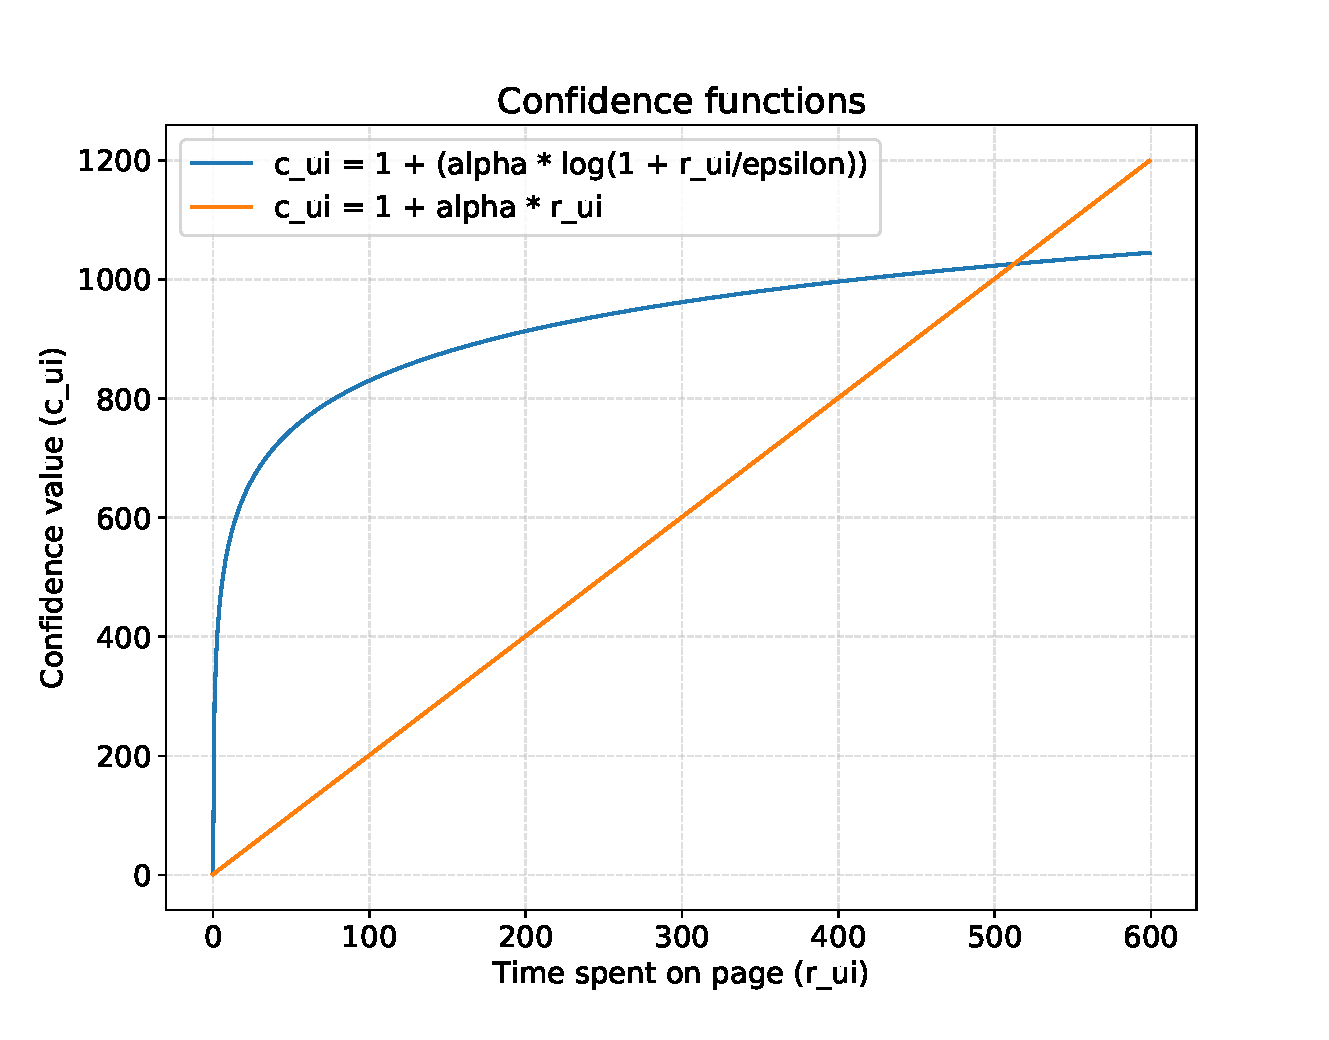
\includegraphics[scale=0.65]{obrazky-figures/confidence2.pdf}
    \caption{This figure visualizes the graphs of the linear \ref{eq:lin_conf} and the logarithmic \ref{eq:log_conf} confidence functions. The linear confidence, colored in orange, used $\alpha=2$. The logarithmic, colored in blue, used $\alpha=120$ and $\epsilon=0.1$.}
\end{figure}
Example of an existing publicly available dataset using implicit feedback could be the~Last.fm \footnote{\url{https://www.dtic.upf.edu/~ocelma/MusicRecommendationDataset/lastfm-360K.html}} dataset. Last.fm \footnote{\url{https://www.last.fm/}} is an online music service and this dataset was used to create music recommendations. It consists of tuples in format \texttt{<userId,itemId,plays>} where \texttt{userId} is a unique user identifier, \texttt{itemId} is a song identifier and \texttt{plays} is the total number of times this user listened to the song.


%===============================================
% Our Dataset
%===============================================
\section{Our Dataset} \label{our_dataset}
The recommender system, that is in the main interest of this thesis, is working with webpages from the \texttt{developers.redhat.com} domain. These webpages contain articles, blog posts and videos not only about the products of the \texttt{Red Hat, Inc.} company but also about several topics across the industry of information technologies.

The dataset consists of records about visits to these webpages. An interaction between a user and a page is therefore just a visit to this webpage. This makes the dataset purely implicit as the system only knows what pages have its users visited but has no idea about what pages they actually liked. There is, however, a numeric value associated with every interaction. A value that embodies an essence of preference and thus helps the system to better understand and evaluate the data. This value is the time that a user spent on a~webpage during his visit. 

Apart from that, every interaction has to carry an identifier of the user and the webpage that was involved in it. Identification of the involved webpage is simply performed by its URL. The identification of a user is done using not one but two values, the \texttt{visitor\_id} and the \texttt{user\_id}. An overall structure of one record (all the values or variables of one record) is as follows:

\begin{itemize}
    \item \texttt{visitor\_id}: This value identifies the cookies that were used in the interaction.
    \item \texttt{user\_id}: Unique identifier assigned to logged in users.
    \item \texttt{page\_url}: URL of the involved webpage.
    \item \texttt{time}: The time in seconds that the user spent on this webpage.
\end{itemize}
Not all interactions in the domain are produced by logged users. In those cases, the \texttt{user\_id} is simply not known and the system has to use only the cookies to identify the source of this action. An example of one record in the dataset can be seen in table \ref{tab:dataset_record}. \\ \\

\begin{table}[h!]
    \centering
    
    \begin{tabular}{ll}
    \hline
    \rowcolor[HTML]{EFEFEF}
    user\_id    & 75296503                                                      \\ 
    visitor\_id & 123456\_987654                                                \\ 
    \rowcolor[HTML]{EFEFEF}
    page\_url   & https://developers.redhat.com/blog/2018/08/29/intro-to-podman \\ 
    time        & 156                                                           \\ \hline
    \end{tabular}

    \caption{Example of one record in the dataset. This record represents an interaction between a user and a webpage in the form of a visit to this webpage.}
    \label{tab:dataset_record}
\end{table}
Our dataset, consisting of records of these interactions collected over 6 months (from September 2018 to February 2019), includes a total of \textbf{265123} interactions.
As it was already mentioned, not all the interactions in the dataset were created by logged users. In~fact, only about 29\% of them know the exact \texttt{user\_id} involved. The rest of them only know the \texttt{visitor\_id} representing the cookies of a browser. 

That means if the system worked only with interactions of logged users, it would be able to use only 76369 interactions from the~original 265123. On the other hand, it would be tricky to use only the \texttt{visitor\_id} to~recognize the user, as cookies identify the browser rather than the users themselves. They can also change over time or be deleted. Or even worse, 2 different people using the same computer would be identified as one user. All of those problems resulted in creating a~mechanism called \texttt{UserMappings}. This mechanism strives to combine both \texttt{user\_id} and \texttt{visitor\_id} to create a unique user identifier. By that, it creates the advantage of being able to connect interactions, where only the \texttt{visitor\_id} is known, to the actual user, once he is logged in and creates new interactions with his \texttt{user\_id}. More details on this topic can be found in section \ref{implementation}.


\subsection*{Metadata} \label{metadata}
A good step to further improving the performance of a recommender could be including an additional piece of information about the items of the system. That means besides the user-item interactions, the system would also have some metadata describing the nature of its users and items.  Assigning every item with a description or tags creates a sort of profile that helps to classify it. Similarly, a profile for users helps to find other similar users and consequently helps to recommend new items. 

User profiles are often created by users themselves and often contain demographic information like age, gender or nationality. Sometimes they let their users to directly determine their preferences e.g. what music genres or what bands they listen to. Item profiles, on the other hand, are created by the system and describe the nature and characteristics of their content. In the \texttt{Movielens} dataset, movies are assigned with genres like Western, War, Thriller, Sci-Fi, Romance etc. This information comes in hand, especially when working with content-based recommenders, that use it to compute similarities between items. 
In~our case, the system can work with the following metadata:

\begin{table}[h!]
    \centering
    \begin{tabular}{@{}ll@{}}
    \toprule
    key         & \multicolumn{1}{c}{value}                                                                                                                                                                                                                               \\ \midrule
    \rowcolor[HTML]{EFEFEF} 
    page\_url   & https://developers.redhat.com/blog/2019/02/26/...                                                                                                                                                                                                       \\
    title       & Creating and deploying a Java 8 runtime container image                                                                                                                                                                                               \\
    \rowcolor[HTML]{EFEFEF} 
    tags        & \begin{tabular}[c]{@{}l@{}}{[}buildah, container, docker, java, java 8, \\ kubernetes, microprofile, openjdk, openshift{]}\end{tabular}                                                                                                \\
    description & \begin{tabular}[c]{@{}l@{}}a java runtime environment should be able to run compiled source code, \\ whereas a development kit, for example, openjdk, would include all \\ the libraries/binaries to compile and run the source code ...\end{tabular} \\ \bottomrule
    \end{tabular}
    \caption{An example of article metadata.}
    \label{tab:additional_info}
\end{table}

The metadata of each item consist of its URL, that also serves as a unique identifier, the \texttt{title} of the article, a list of \texttt{tags} that create a basic form of categorization and were assigned to it by a human and a short \texttt{description}, being the first paragraph of its textual content.


%===============================================
% Approaches
%===============================================
\chapter{Approaches to building Recommender Systems} \label{approaches}
This chapter offers an overview of the most popular methods, used to build recommenders. Section \ref{content_based} starts by describing the principles of content-based approaches. Section \ref{cf_theory} moves on to collaborative filtering methods. Section \ref{hybrid_models} leaves a couple of words about hybrid models and finally, section \ref{deep_learning} describes several methods using deep learning.

%===============================================
% Content-Based
%===============================================
\section{Content-based Models} \label{content_based}

One of the first approaches used to build recommenders were content-based methods. These methods use specific measures to compute similarities between items or users. Then, based on those computed similarities, they are able to make recommendations.
Content-based methods are often classified as either item-oriented or user-oriented:

\begin{itemize}
    \item item-oriented - compute similarities between items, recommend most similar items to those users already liked
    \item user-oriented - compute similarities between users, recommend items liked by similar users.
\end{itemize}
To make such similarity measures possible, the system has to give all items or users a~uniform way of representation. As mentioned in section \ref{metadata}, representation of users can reflect their preferences but also information like their age or gender. It can be either learned by~the~system, as~it observes their interactions, or set directly by the users. The representation of items is often constructed directly from their content. Web articles, for example, can be represented as n-dimensional vectors created using various natural language processing techniques.

More formally, as suggested in paper \cite{Toward}, let $Content(s)$ be the~representation of article $s$. One of the~techniques used to create it is the~term frequency/inverse document frequency (TF-IDF) measure. This measure is used to calculate keyword weights in a~document. The~term frequency of word $i$ in article $j$ is defined as:
\begin{equation}
    TF_{i,j} = \frac{f_{i,j}}{max_{z}f_{z,j}}
\end{equation}
Where $f_{i,j}$ is the number of times word $i$ occurred in article $j$, and $max_{z}f_{z,j}$ is the maximum number of occurrences of a word in article $j$. This measure, however, has a small flaw. It~gives big values to words commonly used in the language. These words do not have any importance in defining the articles, because they do not describe their content. Therefore the inverse document frequency (IDF) measure is added. The inverse document frequency for word $i$ is defined as: 
\begin{equation}
    IDF_{i} = \log \left( \frac{N}{n_{i}}\right)    
\end{equation}
Where $N$ is the number of all articles in the dataset, and $n_{i}$ is the number of articles in which the word $i$ appeared. If a word appears in every article, its $IDF$ value is 0. Such a word does not represent any special feature and therefore cannot be used to describe an article. On the other hand, if a word is used only in a few articles, its significance is bigger and so is its $IDF$ value. The final weight of the word $i$ in article $j$ is then computed as: 
\begin{equation}
    w_{i,j} = TF_{i,j} \times IDF_{i}
\end{equation}
And the content of article $s$ is represented as a vector of these weights:
$$Content(s) = (w_{1s}, ..., w_{ks})$$
Finally, the similarity of two articles $c$ and $s$, is computed from their content vectors, using some scoring heuristic, such as the cosine similarity:

\begin{equation}
    sim(c, s) = \cos (\Vec{w}_{c}, \Vec{w}_{s}) = \frac{\Vec{w}_{c} \Vec{w}_{s}}{||\Vec{w}_{c}|| \: ||\Vec{w}_{s}||}
\end{equation}
Where $\Vec{w}_{c}$ is the content vector of article $c$ and $\Vec{w}_{s}$ is the content vector of article $s$. The~$||\Vec{w}_{c}||$ term stands for the Euclidean $L^2$ norm of vector $\Vec{w}_{c}$. The similarity is given by the cosine of the angle between the two vectors. This equation originates in the scalar projection of two Euclidean vectors, visualized in figure \ref{scalar_projection}. 

\begin{figure}[H]
    \centering
    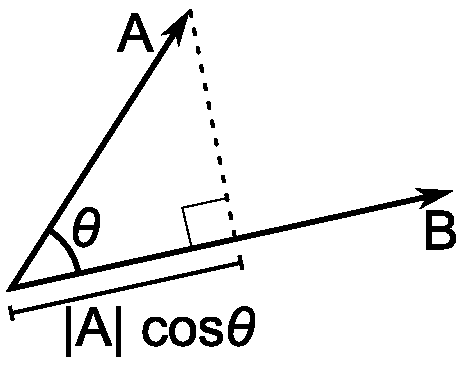
\includegraphics[scale=0.8]{obrazky-figures/dot_product.pdf}
    \caption{Scalar projection of vector $A$ in the direction of vector $B$.}
    \label{scalar_projection}
\end{figure}

Having vectors $a$ and $b$, the scalar projection of vector $a$ in the direction of vector $b$ is given by:

\begin{equation}
    a_{b} = ||\Vec{a}|| \ cos(\Theta)
\end{equation}
Where $\Theta$ is the angle between the two vectors. The dot product of the two vectors can be thus characterized geometrically as:

\begin{align}
    \Vec{a} \cdot \Vec{b} & = ||\Vec{b}|| \ a_{b}  \\
    \Vec{a} \cdot \Vec{b} & = ||\Vec{b}|| \ ||\Vec{a}|| \ cos(\Theta)
\end{align}
When this equation is solved for the $cos(\Theta)$ term, it becomes the cosine similarity equation. 

Another example of creating item profiles could be using some document embedding method such as Doc2Vec, introduced in 2014 by Le and Mikolov in paper \cite{Doc2Vec}, or a sentence embedding method called InferSent \cite{InferSent}. These methods use complex NLP approaches to create vector representations of text-based data in a joint n-dimensional space, in which similar items are placed close to each other. The recommendation task would then consist only of finding the most similar vectors, that is the ones being closest to a certain vector, which could be easily done by taking the dot product of the two vectors.


One problem that these models encounter is recommending items to new users when no user-profiles are available. Another problem can be in the recommendations themselves. The system may keep recommending articles from the same area, or about the same topic all over again, just because they are similar. This may cause a problem sometimes called the~\texttt{information bubble}. Users would not be recommended any new topics or genres outside the space of their own bubble, rendering the system useless in terms of discovering new interests.

%===============================================
% Collaborative Filtering
%===============================================
\section{Collaborative Filtering} \label{cf_theory}

A more recent approach to recommendations is presented by collaborative filtering models. Content-based models use specific techniques to recommend the most similar items. However, this strategy can cause the system to isolate its users, preventing them from discovering new topics and interests. 

Collaborative models try to overcome this problem by incorporating collaborative information into the recommendations. When these models compute preferences, they do not look only at interactions of one user. They look at the interactions of other users as well. For example, as mentioned in article \cite{GoogleCloud}, if user 1 liked articles A, B, C, D, E and user 2 liked articles A, B, D, E but not C, the collaborative model would look at both users and see this connection. Then, user 2 would be recommended article C, even if the article was not similar to those he already liked. These models rely only on observed behaviour, thus there is no need to create user or item profiles as it was in content-based models.



\subsection{Neighbourhood Models}

Neighbourhood models represent one of the most common approaches to collaborative filtering. They use a strategy similar to content-based (CB) models and are also classified as user, or item-oriented. Unlike CB models though, they do not only recommend the most similar items. They predict the rating of an item, based on its most similar items, also known as neighbours, and then recommend those with the highest predicted ratings. The~prediction can be done by performing a weighted arithmetic mean over the ratings of the most similar items, with the weights being the measured similarities. Then, as suggested in paper \cite{Implicit}, for user $u$ and item $i$ the~predicted rating $r_{ui}$ is given by:
\begin{equation}
    r_{ui} = \frac{\sum_{j \in S^k_{(i,u)}}(s_{ij}r_{uj})}{\sum_{j \in S^k_{(i,u)}} (s_{ij})}
\end{equation}
Where $S^k_{(i,u)}$ is the set of $k$ most similar items to item $i$ that were rated by user $u$, and $s_{ij}$ is the computed similarity between items $i$ and $j$. Similarly, the rating could also be computed as a weighted average of ratings, most similar users gave this item. The~Neighbourhood models are suitable mainly for explicit feedback datasets, as their ratings are still on the same scale. Whereas with implicit feedback the system often works with frequencies that have different scales, depending on the application.


\subsection{Latent Factor Models} \label{latent_factor_models}

Latent factor models represent a different approach to collaborative filtering. These models assign all users and items with n-dimensional vectors and try to discover latent features, that explain the observed interactions, in them. These latent features represent hidden attributes that describe the properties and characteristics of users and items. 

For web articles, these attributes could be e.g. how much does an article resemble a~certain topic, where each dimension of its vector would be the weight of one topic, how recent the article is etc. The vector of a user then represents the importance that the user gives to these attributes. If the user really likes articles about machine learning, then the value representing this attribute will be bigger. These latent attributes, however, are only hypothetical. We do not know what attributes the dimensions of vectors represent. That~is why they are called latent or hidden. They are learned by the system. Examples of these models include LDA and SVD. 

Latent factor models are often implemented using the \textbf{matrix factorization} method. This method gained its popularity because of its simplicity and the ability to operate with different types of input data, of both explicit and implicit datasets. The first step of this method is to put the input into a matrix, with one dimension representing users and the other representing items. The corresponding fields then represent the values of interactions between users and items, e.g. a rating a user gave to an item.

\begin{figure}[H]
    \centering
    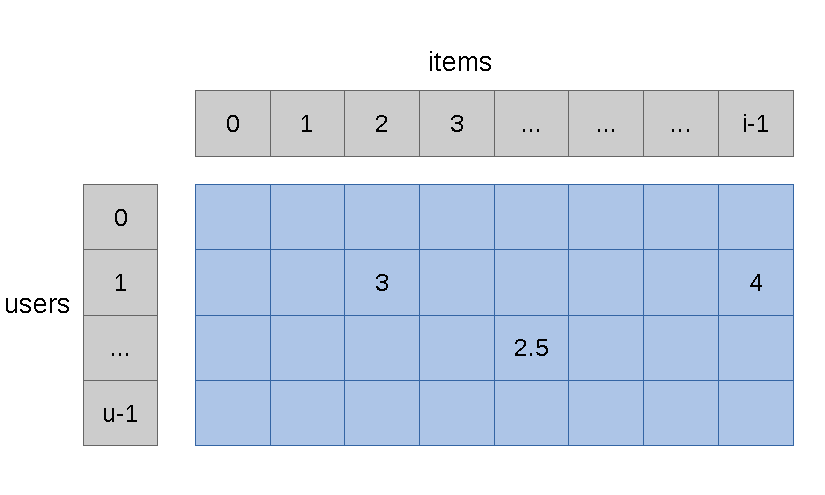
\includegraphics{obrazky-figures/matrix.pdf}
    \caption{Example of an interaction matrix with explicit feedback. Values in the matrix represent the ratings users gave certain items. \cite{GoogleCloud}}
    \label{Matrix}
\end{figure}

As told in article \cite{MF}, these methods map both users and items to a joint latent factor space of dimensionality $n$, such that user-item interactions are modelled as the inner product in that space. That means the model creates two matrices. The first that contains n-dimensional vector for every user and the second that contains vectors of the same dimensionality for all items. Then the system infers these vectors so that when it takes the inner product of a user and an item, it gets the corresponding interaction value from the~original matrix. Therefore the multiplication of the two matrices is an approximation of the original matrix, as visualized in figure \ref{Factorization}

\begin{figure}[H]
    \centering
    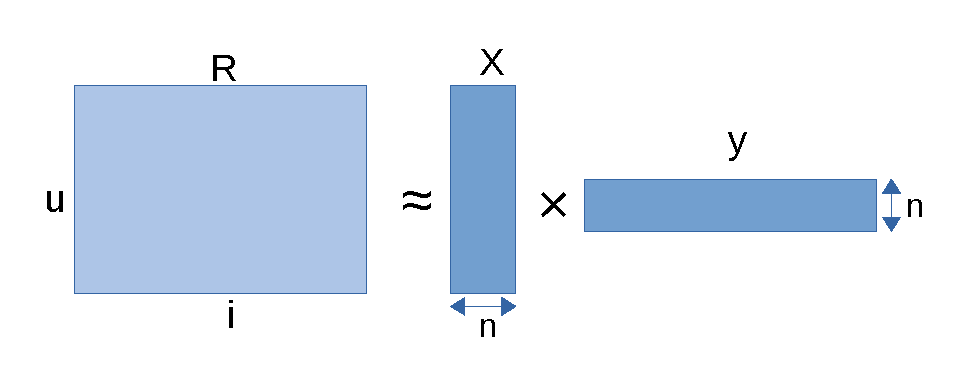
\includegraphics[scale=0.9]{obrazky-figures/factorization.pdf}
    \caption{$R$ is the interaction matrix, $X$ contains n-dimensional vectors of users, $y$ contains vectors of items, $u$ is the number of users and $i$ the number of items in the dataset. Multiplication of $X$ and $y$ is an approximation of the original matrix $R$. \cite{GoogleCloud}}
    \label{Factorization}
\end{figure}

This process can be also explained as compressing the sparse matrix R into much lower n-dimensional space. In this space, every user and every item is represented as a vector of latent factors, with each dimension being the significance of one factor. The rating $\hat{r}_{ui}$ user $u$ gave item $i$ is then calculated as the inner product of their vectors:
\begin{equation}
    \hat{r}_{ui} = x_{u}^T y_{i}
\end{equation}
Where $x_{u}$ is the vector of user $u$ and $y_i$ the vector of item $i$.
More precisely, this is an approximation of the actual rating. To find the correct representation of these vectors, the system defines a loss function $L$:

\begin{equation}
    L = \sum_{u,i} (r_{ui} - x_{u}^T y_{i})^2
\end{equation}
Where $r_{ui}$ is the actual rating.
To train the model and find the vectors, the system has to minimize this loss function. It is a common practice to add an L2 regularization term to prevent overfitting. Then the loss to minimize is defined as:

\begin{equation}
    L = \sum_{\text{known}\ r_{ui}} \quad (r_{ui} - x_{u}^T y_{i})^2 + \lambda (||x_{u}||^2 + ||y_{i}||^2)
\end{equation}
Where $\lambda$ is a regularization constant, that is one of the hyperparameters of the model. This~loss is usually computed only on known observations.
These equations, however, only apply to explicit feedback, where the $r_{ui}$ values are on~a~fixed scale. To be able to use matrix factorization techniques on implicit feedback, some changes need to be made, on these equations. As it was already stated in section \ref{implicit_datasets}, models, that work with implicit feedback, define new variables to describe interactions. In our case, the numerical value of interaction between user $u$ and article $i$, $r_{ui}$, is the time this user spent on the article’s webpage. The~numeric value is then interpreted by two variables. The first one $p_{ui}$, symbolises preference and is a binary representation of the $r_{ui}$ value, as outlined in \ref{eq:implicit_preference}. The second $c_{ui}$ indicates the level of confidence, the system has about the preference of user $u$ toward item $i$. The confidence can be computed as proposed in \ref{eq:lin_conf}, or \ref{eq:log_conf}. Accordingly, the loss function of matrix factorization is computed, using these new variables, as proposed in paper \cite{Implicit}:

\begin{equation}
    L = \sum_{u,i} \quad c_{ui} (p_{ui} - x_{u}^T y_{i})^2 + \lambda (||x_{u}||^2 + ||y_{i}||^2)
\end{equation}
Where $\lambda (||x_{u}||^2 + ||y_{i}||^2)$ is the regularization term, preventing overfitting, $\lambda$ is a data-dependent hyperparameter, learned by cross-validation. Opposed to explicit feedback, the loss function received several changes. First, the preference computed as the inner product of user $u$ and article $i$ now refers to $p_{ui}$ instead of $r_{ui}$. Second, optimization should account for all $u,i$ pairs, rather than only those of known interactions.

Minimization of the loss function is performed using an optimization algorithm. As discussed in~\cite{MF}, explicit feedback models widely use the stochastic gradient descent. Moreover, implicit models often use the \textbf{alternating least squares} (ALS) algorithm. This algorithm alternates between optimizing user-factors $x_{u}$ and item-factors $y_{i}$. Each step it fixes one of these factors and optimizes the other. When all user factors $x_{u}$ are fixed, it optimizes all item-factors $y_{i}$, by solving a least-squares problem, and vice versa.


\subsection*{Singular Value Decomposition}
Another example of matrix factorization is the \textbf{singular value decomposition} (SVD) method. As a generalization of eigenvalue decomposition, it is capable of performing a factorization of a real or complex non-square matrix, decomposing into three different matrices consisting of eigenvectors and eigenvalues. 

This method is of a similar manner as principal component analysis (PCA). In fact, it is equivalent to performing PCA on the covariance matrix of the dataset. A covariance matrix is a square matrix that contains variance and covariance values between the factors of the dataset. PCA is used to find the components of the data that have the biggest variance, as shown in figure \ref{pca}.

SVD performs a factorization of a matrix into three matrices. Given an $m \times n$ matrix $M$, the SVD of $M$ would be in the form of:

$$ M = U \Sigma V^\text{T} $$
Where the created matrices are:
\begin{itemize}
    \item $U$: Eigenvectors of $M M^\text{T}$.
    \item $\Sigma$: A diagonal square matrix, containing so-called singular values of matrix M. These are the square roots of eigenvalues of both $M M^\text{T}$ and $M^\text{T} M$.
    \item $V$: Eigenvectors of $M^\text{T} M$.
\end{itemize}
In our case, $M$ is the interaction matrix. After performing SVD, matrix $U$ represents latent features of users, $V$ represents features of items and $S$ is a diagonal matrix giving the~relative significance of these factors. The user-item interactions are once again modelled as the inner product of a user vector from matrix $U$ and an item vector from matrix $V$:

$$r_{ui} = U_{u} \cdot V_{i}$$
SVD is mainly used for dimensionality reduction tasks. The generated matrix $\Sigma$ is actually a diagonal matrix with eigenvalues, that express the variance or significance in corresponding dimensions. Dimensions with small eigenvalues can thus be excluded as they carry a negligible amount of information. In recommendation tasks, however, the goal is not to reduce dimensionality. The intention is to fill in the missing values of the sparse matrix, which basically means predict the missing interactions. The usage of SVD for recommendation can be found in \cite{SVD}.

\begin{figure}[H]
    \centering
    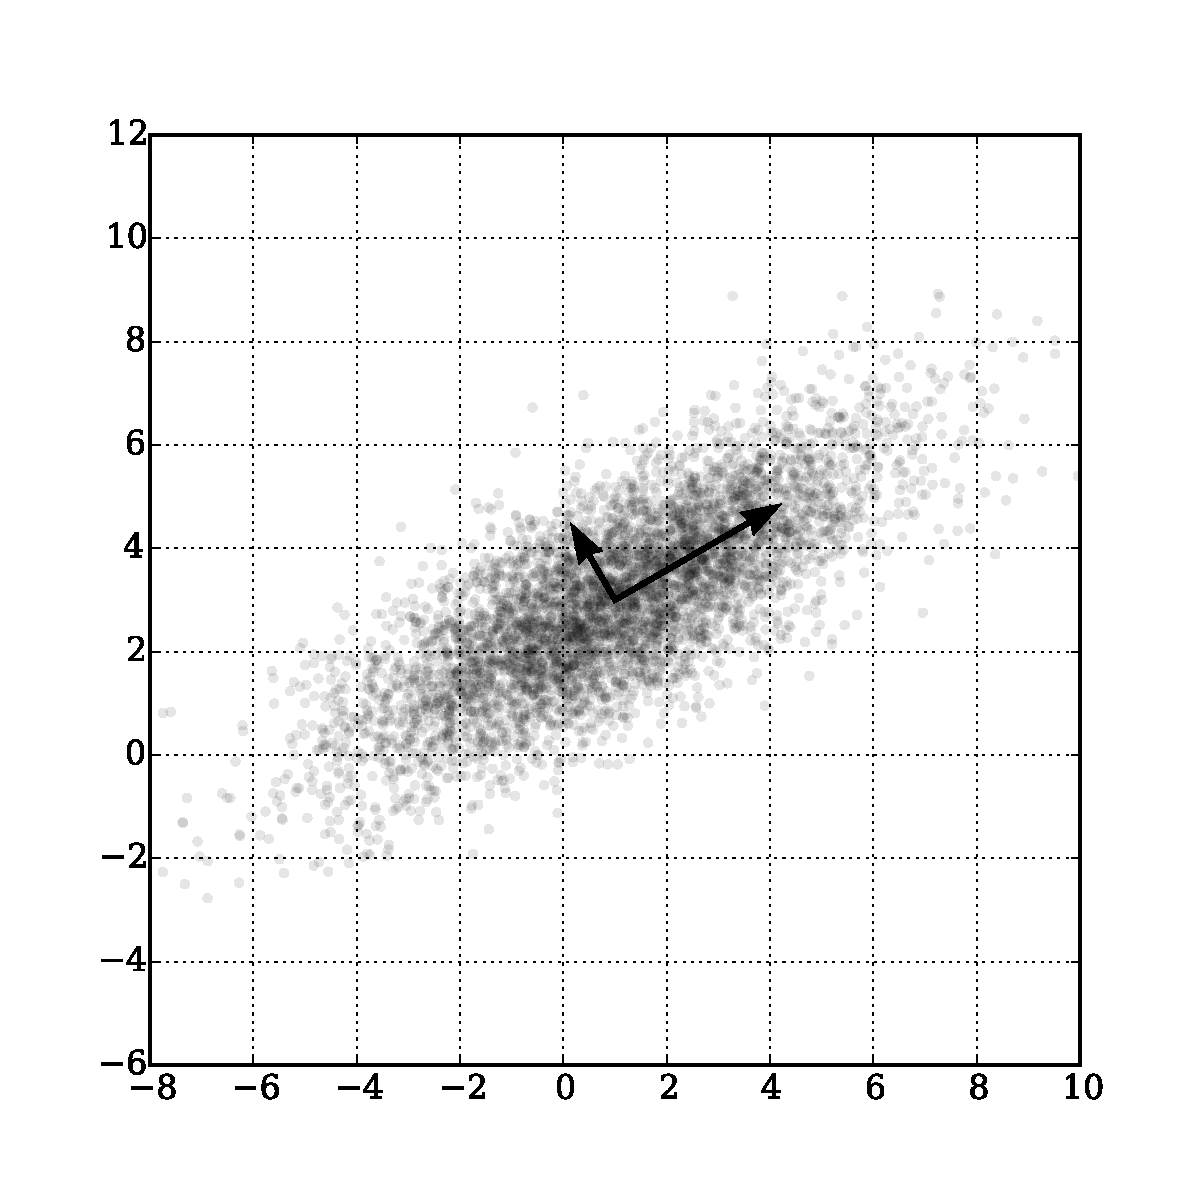
\includegraphics[scale=0.48]{obrazky-figures/pca.pdf}
    \caption{Principal component analysis of a Gaussian distribution. The vectors shown, are the eigenvectors with the biggest eigenvalues. Their eigenvalues are placed in the first and the second position in the diagonal covariance matrix. The vectors are pointing to the two directions with the biggest variances. Taken~from:~\textit{https://commons.wikimedia.org/wiki/File:GaussianScatterPCA.svg}.}
    \label{pca}
\end{figure}


\subsection*{Cold-start problem}
The cold-start problem is a term used to define a state in the system where very few records of user-item interactions are present. It also occurs when a new user, that has not created any interactions yet, comes to the system. And similarly when new items come to the system and with no users interacting with them. The performance of collaborative models in such an environment is very poor. It is possible, however, to boost the model with some other technique that is more proficient in these situations. A traditional content-based model, for example, is able to find similarities without the need of having known any actual interactions, using metadata in user or item profiles. This strategy of combining two methods results in so-called \texttt{Hybrid models}.


\section{Hybrid Models} \label{hybrid_models}

Hybrid models strive to combine the strengths of both content-based (CB) and collaborative filtering (CF) methods. The main reason for their existence is to eliminate the cold-start problem and at the same time preserve the good performance of collaborative models. An~example of a hybrid model is described in paper \cite{LightFM} by Maciej Kula. 
The~main objectives of hybrid models can be summed as:

\begin{itemize}
    \item In cold-start and low-density scenarios, they profit from CB techniques, therefore items can be recommended using the computed similarities between their profiles.
    
    \item When the interaction matrix is dense, they incorporate collaborative information and boost the performance of the model, using CF techniques.
\end{itemize}


%===============================================
% Deep Learning
%===============================================
\section{Deep Learning Models} \label{deep_learning}
Deep learning represents a special segment of non-linear probabilistic models that use artificial neural networks. These models use multiple layers of computational units to extract high-level features from data. Due to the huge momentum in deep learning research over the past few years, these methods found their way into various spheres of the industry and recommender systems are not an exception. 

Some of the earlier architectures introduced the usage of Restricted Boltzmann Machines for collaborative filtering \cite{Boltzmann}. The usage of deep learning in content-based methods followed soon after, as it is often used to learn vector representations based on the content of objects. Whether it is images or textual data that the network is learning to represent, the task of recommenders remains the same: find the most similar items. As this thesis works with web articles, it is reasonable to focus mainly on textual based data. Several Natural Language Processing (NLP) architectures strive to create text embeddings, such as Doc2vec \cite{Doc2Vec} or Infersent \cite{InferSent}. Finding the similarities of items can be then simply completed by taking the dot product of their vectors.

Another architecture, described in \cite{Convolutional}, uses convolutional neural networks to predict the future behaviour of users based on the sequence of their past interactions. It models each user by embedding this sequence of recent items into a matrix representing an “image”. Then, similarly to image processing, it uses convolutional filters to learn the sequential patterns as local features of the image. Such recommendations, however, are very temporary and case specific. The predictions are relevant only at that exact moment in one particular sequence and hence cannot be used in later times. 

A similar approach is held by so-called Session-based recommender systems, that also operate only with a sequence of the most recent interactions created in one single session. This session can be for example an internet session, meaning all the interactions made during one visit of a certain domain. One such architecture \cite{Session-based}, uses recurrent neural networks (RNNs) with slight modifications to traditional RNNs, such as a ranking loss function designed for this problem. More on this topic can be found in \cite{Session-based_Survey}. 

A different but not less popular approach uses a combination of jointly trained wide linear model and a deep neural network. This Wide\&Deep learning model was introduced in \cite{Wide&Deep} and similarly in \cite{DeepFM}, \cite{xDeepFM}. 

Another group of methods tries to go beyond the limitations of using linear models for the task of collaborative filtering (CF). Instead, these methods propose to use non-linear probabilistic models, such as deep autoencoders \cite{Autoencoder} or variational autoencoders \cite{vae_for_cf}, to overcome these limitations and improve the performance of CF techniques.

\subsection*{Doc2Vec} \label{doc2vec_description}
Doc2Vec is a method used to generate numerical representations of documents, that preserve the semantic characteristics of their content. Such representations could be then used for several tasks including web search, spam filtering etc. The architecture of this model is actually very similar to the Word2Vec model. In fact, it uses nearly the same algorithms to which it adds a new vector called ParagraphID. The ParagraphID, also called paragraph vector, represents one particular document. They are placed in a separate matrix and are learned during the training on predicting words from the text of their document. 

The Word2Vec method distinguishes between two versions of the model, each using a slightly different approach to create the word vectors. The first one is called the Skip-gram model. In this version the word vectors are trained by predicting the context of a given target word. The other version, called Continuous bag of words (CBOW), goes the other way around. It takes the context words, either concatenates them, or finds their average, and learns to predict the target word. The Doc2Vec model modifies these two methods of Word2Vec, by adding the paragraph vector. A more detailed description of the Skip-gram model can be found in section \ref{proposed}.


\begin{figure}[H]
    \centering
    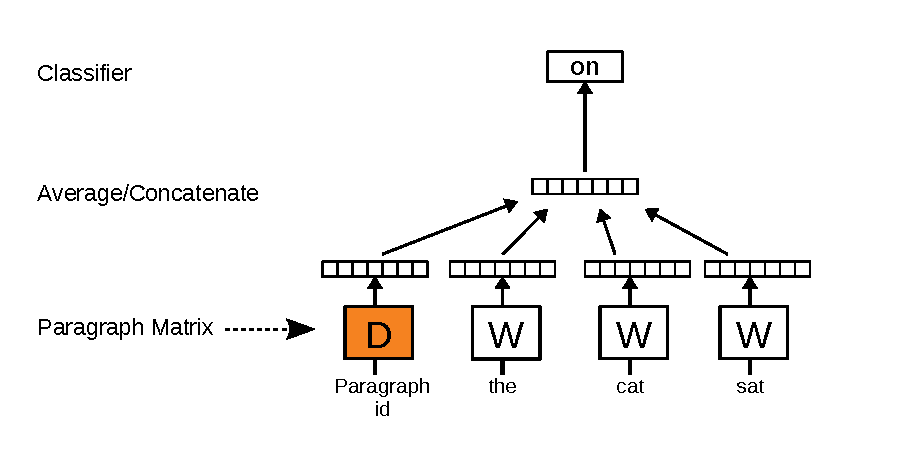
\includegraphics[scale=0.8]{obrazky-figures/pv-dm.pdf}
    \caption{PV-DM algorithm of Doc2Vec. \cite{Doc2Vec}}
\end{figure}

The version based on CBOW is called Distributed memory (PV-DM). In fact, it only adds the paragraph vector to the context vectors, whose sum, or average, is used for predicting the target word. The other version, called Distributed bag of words (DBOW), is a modification of Skip-gram. Here the paragraph vector is used to predict the context words from a randomly sampled window in the corresponding document.

\begin{figure}[H]
    \centering
    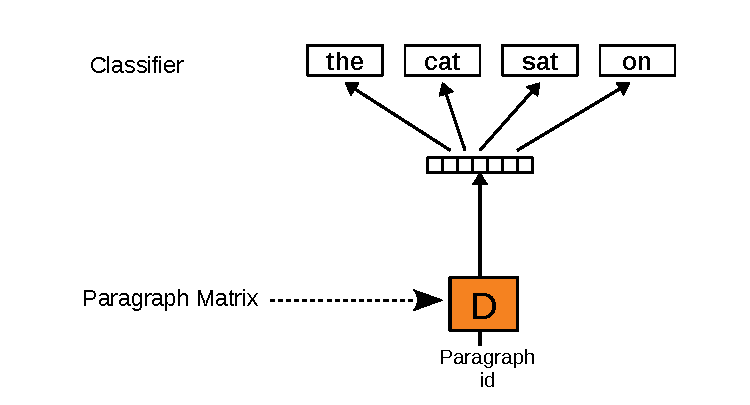
\includegraphics[scale=0.8]{obrazky-figures/pv-dbow.pdf}
    \caption{PV-DBOW algorithm of Doc2Vec. \cite{Doc2Vec}}
\end{figure}

As the publication of Doc2Vec dates back to the year 2014, it is clear that it no longer is a state-of-the-art method for most of the NLP tasks. The reason why it was chosen for this thesis, lies mainly in its simplicity and familiarity. It could be appropriate to try a newer approach in future work. Such as a recently published sentence embedding method called Infersent, described in paper \cite{InferSent}.


%===============================================
% Evaluation Theory
%===============================================
\chapter{Evaluation metrics} \label{eval_metrics}
All the evaluation metrics, used in this thesis, are implemented within the \texttt{Evaluator} class, specified in section \ref{class_model}. All of these metrics are based on techniques that have been previously applied to the problem of evaluating recommender systems and hence should provide a valuable reference to the effectiveness of those models. The particular metrics that were used are the RANK evaluation, Recall at k and Precision at k. Each of them treating the problem in a slightly different way. Following is a more detailed description of each of these techniques.

\section{RANK}
This technique is based on the original RANK metric proposed in paper \cite{Implicit}. It was designed with the intention of evaluating effectively recommenders working with implicit feedback. Therefore it is considered to be one of the most suitable approaches for this task. 

The original paper requires the system to provide all users with an ordered list containing their recommended items, with these items being sorted in descending order by the computed score of preference. That means, that items situated at the beginning of the list are predicted to be the most suitable, and items at the end of the list are the least suitable for that particular user. The paper then denotes a new variable called $rank_{ui}$. This variable expresses the percentile ranking of the position of item $i$ within the ordered list of recommended items for user $u$.

Where the item that lies at the first position in the list, meaning it was predicted to be the most suitable for this user, has the $rank_{ui}$ value assigned to 0\%, whereas an item at the very end of the list, as the least suitable one, has a $rank_{ui}$ value of 100\%. Then, with the $rank_{ui}$ defined, the value expressing the quality of the created recommendations is computed as:

\begin{equation}
    RANK = \frac{\sum_{u,i} r_{ui} \cdot rank_{ui}}{\sum_{u,i} r_{ui}}
\end{equation}
Where $r_{ui}$ is the numeric value of the interaction between user u and item i. In this case, $r_{ui}$ is the time user u spent on the webpage of article i. A good-working recommender system should place items with big $r_{ui}$ values close to the top in the list of recommendations. In fact, the bigger the $r_{ui}$ value, the higher the position should be and hence the lower the corresponding $rank_{ui}$ value. The range of possible values of this metric is 0-100\%. The~lower the RANK the better the system is. If the RANK value is >= 50\% the system is no better than a system with uniform distribution. \cite{Implicit}

\section{Precision at k}
This metric represents a commonly used approach in the area of evaluating recommender systems. However, it is known to be more suitable to systems working with explicit feedback, where users have the ability to express both their positive and negative preference. To~clearly understand the process of this metric, it is important to know the distinction between recommended and relevant items. Recommended items are simply those that were predicted by the system to be the most suitable for a certain user. In terms of the precision at k, the measure looks at the top k recommended items. The definition of relevant items can differ from one system to another. In a system that works with explicit ratings on a scale of 0-5, relevant items could be those that were given a rating of at least 3.5. In terms of an implicit dataset, relevant items for a user are usually all those he interacted with. 

This metric looks at the top k created recommendations to find out how many of them are actually relevant to the user. The relevant items that are used for evaluation are only those occurring in interactions from the test set. Meaning those that the system was not trained on and therefore does not know they are actually relevant. The precision metric can be formally defined as:

\begin{equation}
    \text{precision} = \frac{{S_u}^k \cap {R_u}^t}{k}
\end{equation}
Where ${S_u}^k$ is a list of top $k$ recommended items for user $u$, k is the number of retrieved recommendations and ${R_u}^t$ are the relevant items from the test set, for user $u$. Unlike in the RANK evaluation metric, here the bigger the precision, the better the system is. The range of its values is from 0 to 1. That means, when multiplied by 100, it represents the percentage of relevant items among the top k recommendations.

\section{Recall at k}
This metric is very similar to the above-described precision metric. As it was already mentioned, the precision at k metric and precision metrics, in general, are not very suitable for recommender systems that are designed to work with implicit feedback. Recall metrics, however, try to overcome this obstacle. The recall at k metric modifies the precision, by dividing the number of relevant items among the recommended, not by k, but by the number of all relevant items for user u.

\begin{equation}
    \text{recall} = \frac{{S_u}^k \cap {R_u}^t}{|{R_u}^t|}
\end{equation}
Where ${S_u}^k$ is the list of top $k$ recommendations, ${R_u}^t$ are the relevant items for user $u$ in the test set and $|{R_u}^t|$  is the number of them. This metric actually expresses the percentage of all relevant items in the top k recommendations.


%===============================================
% Proposed Method
%===============================================
\chapter{Proposed Method} \label{proposed}
The intention of this chapter is to describe the proposed architecture, that was developed as one of the models implemented in this thesis. The objective was to implement an architecture based on a probabilistic model that had not been used for this task before and to prove that it can compete with the conventional methods using traditional machine learning algorithms. Hence for these arguments, the SkipGramRecommender is proposed as a neural network recommendation system based on the Skip-gram model, presented in the Word2Vec paper \cite{Word2Vec} and used in the model itself.

\begin{figure}[H]
    \centering
    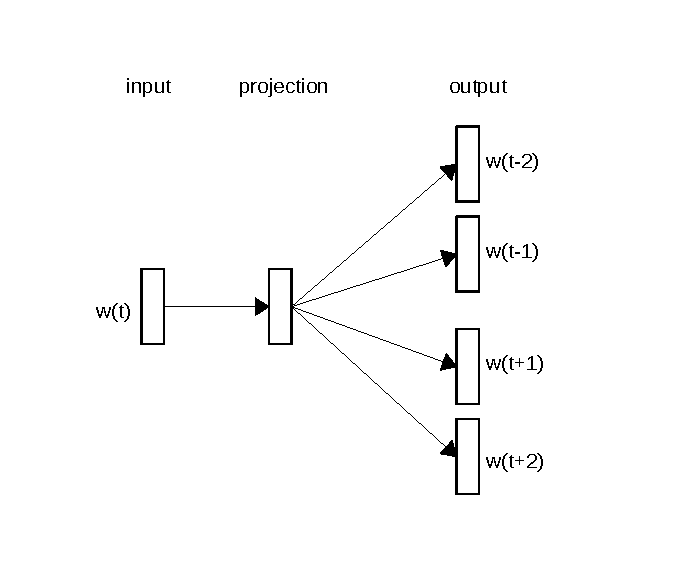
\includegraphics[scale=0.8]{obrazky-figures/skipgram.pdf}
    \caption{Word2Vec Skip-gram model learns to predict the context words of a given target word. Here, $w_{(t)}$ is the target word on position $t$ in the corpus text, $w_{(t+1)}$ is the context word one place ahead of the target word, $w_{(t-1)}$ is the context word one place behind the target etc. \cite{Word2Vec}}
\end{figure}

The Word2Vec is a technique consisting of a shallow, two-layer neural network, that is used to create vector representations of words also known as word embeddings. The goal of such representations is to allow the system to be able to see semantic relations among those words. By assigning vectors to words it projects them into a joint multidimensional space where words, that share common contexts in the corpus text, are positioned close to each other. The vectors are being learned as the system is trying to predict words that lie in the context of a given target word. One of the methods, used for this task, is implemented by the Skip-gram model. 

In the connection to the Skip-gram model, a popular analogy of a sliding window is often used. This analogy explains the process as if a window of size n, is sliding over the words as they lie in the corpus text one after another, to create an input for the network. Each time, one word from this window is chosen to be the target word. The other words from the window are then the context words. The algorithm then learns to correctly predict the context words, given the target word, that means to assign those words with bigger probabilities that they lie in the close surrounding of the target word. It does so by maximizing the dot product of surrounding word representations with target word representations. Hence for words with similar context end up being positioned close to each other in the resulting space.

\begin{figure}[H]
    \centering
    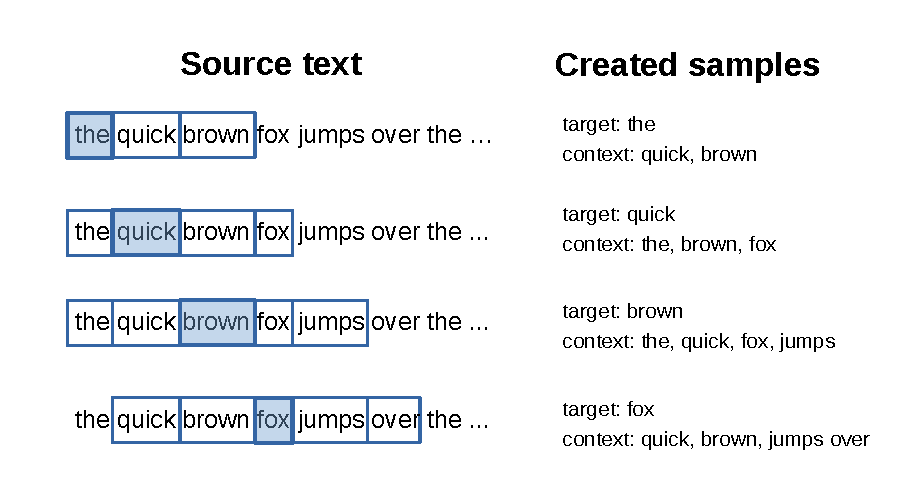
\includegraphics{obrazky-figures/sliding_window.pdf}
    \caption{This figure shows how training input for the Skip-gram model is created. It~uses the analogy of a sliding window of size 2, meaning it takes two words to the left and two words to the right of the target word. The system then learns to predict the context words given a target word. \cite{Sliding_figure}}
\end{figure}

The goal of the Skip-gram method is to find such representations of words, that are useful for predicting the surrounding context words given a target word. Hence for the objective is to maximize the average log probability:

\begin{equation} \label{eq:skip-gram}
    \frac{1}{T} \sum_{t=1}^T \sum_{-c <= j <= c; \, j \neq 0} log \, p(w_{t+j} | w_t)
\end{equation}
Where $c$ is the size of the training context or the context window, given a target word $w_t$, and $T$ is the number of training words.
However, if the model would have to predict all the probabilities for all the words in the corpus, it would take a great number of resources. Therefore a more computationally-efficient modification was created. This new algorithm is called negative sampling.
In this modification, the prediction is not done on all but only on a few randomly chosen negative samples along with the words from the context. A negative sample stands for a word that does not belong to the context of the given target word. The~algorithm then learns to predict the negative samples to be less probable and place them further in the vector space. Authors of paper \cite{Skip-gram} proposed the following expression, that replaces the $log \, p(w_{t+j} | w_t)$ term in the original \ref{eq:skip-gram} objective of Skip-gram:

\begin{equation} \label{eq:neg_sampling}
    log \, \sigma ({{v'}_{w_0}}^T v_{w_I}) + \sum_{i=1}^k \mathbb{E}_{w_i \sim P_n(w)} \Big[log \, \sigma (-{{v'}_{w_i}}^T v_{w_I})\Big]
\end{equation}
Where ${v’}_{w_0}$ is an output vector of a context word $w_0$, $v_{w_I}$ is a vector of a target word $w_I$, $k$ is the number of negative samples and P represents a noise distribution. 
As already mentioned this method is used to create word embeddings. Now it is time to look at the analogies with the recommendation problem that this thesis is dealing with. 
In our case, the system is not dealing with words, but with users and items. However, the task can still be interpreted in a similar manner, that is: place similar items and users close to each other. Looking at the equation \ref{eq:neg_sampling}, the target word can be replaced with a target item. The words from the context window are the users that actually interacted with this item and the negative samples are users that did not. By adjusting the original equation given these analogies, it can be rewritten as:

\begin{equation} \label{our_ns}
    log \, \sigma ({v_{u}}^T v_I) + \sum_{i=1}^k \Big[ log \, \sigma ({-v_i}^T v_I) \Big]
\end{equation}
Where $v_u$ is the context vector representing user $u$ that interacted with item $I$, $v_I$ is the vector of the target item $I$, $v_i$ is the negative sample, meaning a user that did not interact with item I, and $k$ is the number of used negative samples.

By applying this loss function to the recommendation problem the model should, as a result, construct a vector space that incorporates the proximity of common contexts, just like it does with words in the original Word2Vec model.

\section*{The Architecture}
The overall architecture itself contains a few tweaks and enhancements. It does not start off by representing items and users as random vectors. It uses the obtained metadata, mentioned in \ref{metadata}, that describe the content of our items. The construction of an item vector consists of two parts.

First of all, it uses the tags presented in section \ref{metadata}. These tags consist of keywords that were assigned to articles to describe their content and provide a basic form of categorization. Every item was assigned a number of tags. The system takes the most frequently used ones and creates randomly initialized embeddings for them. Every item is then represented as a sum of its tag embeddings, or zeros if none of its tags is known. This is the first part of the construction. 

The second part of it consists of document vectors. The document vectors represent the actual content of items as they are created using models like the already mentioned Doc2Vec, that is further discussed in \ref{doc2vec_description}. The document vector of an item is created from its title and description. These two parts are concatenated together to create the final item\_vector representation. The whole process is depicted in figure \ref{embed_construct}.

\begin{figure}[H]
    \centering
    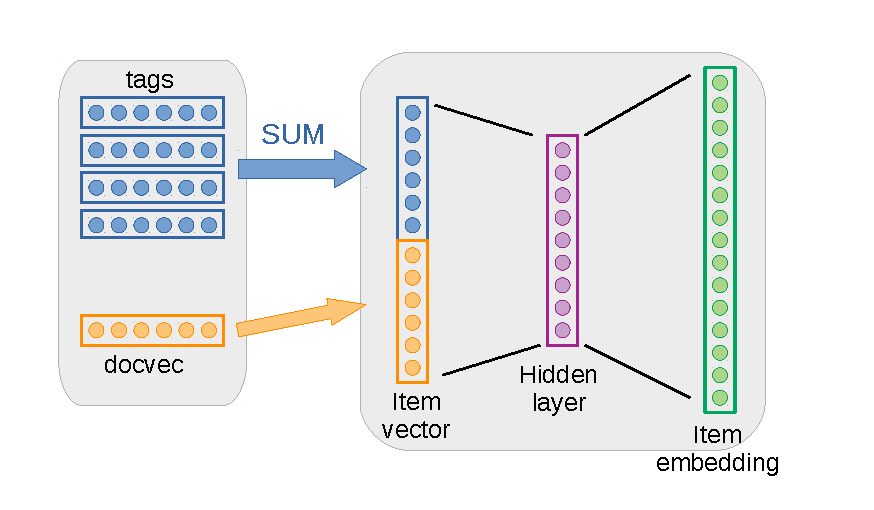
\includegraphics{obrazky-figures/embeddings_construction.pdf}
    \caption{This figure shows the construction of item vectors. The blue dots represent tag embeddings, the orange dots represent a document vector. To construct an item vector, that can be sent into the network, the system takes all embeddings of its tags and sums them into one. Then the system takes the precomputed document vector of this item and concatenates it to the sum. The concatenated vector can then be fed into the network.}
    \label{embed_construct}
\end{figure}

After the construction of item vectors, they are fed into the shallow, two-layer neural network to create the item embeddings. Looking at the equation \ref{our_ns} one can see that except for the item vectors, it is working with user vectors as well. They are constructed directly from items. Every user vector is created as a sum of item vectors that this user actually interacted with.

Following that, the user vector is also fed into the network and the user embedding is created. When all the required parts are ready, the loss function can be computed. As~the model evaluates the loss it backpropagates the computed gradients to learn the best weights for its two layers and also the tag embeddings. The document vectors, representing the second part of the concatenated item vector, are fixed and hence the backpropagation does not change their values.

When the model is trained, the prediction is simply done by generating the corresponding item and user embeddings and performing the dot product of them. To generate the embeddings, the system simply creates both the required item and user vectors and feeds them into the network. To recommend a user with top n items, that are most suitable for him, the system takes the dot product of his embedding with the whole matrix of precomputed item embeddings and returns a list of n sorted items, in descending order according to the results of the dot product. 


\begin{figure}[H]
    \centering
    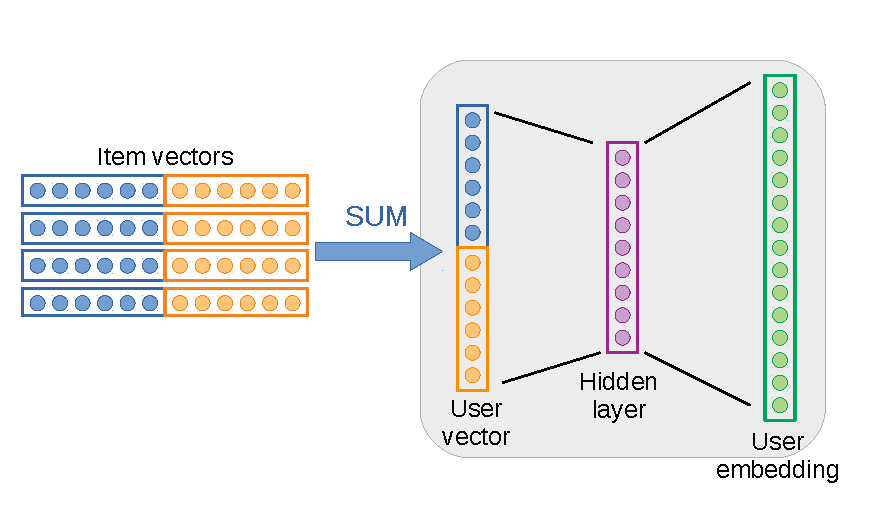
\includegraphics{obrazky-figures/user_embeddings.pdf}
    \caption{This figure shows the construction of a user vector. A user vector is simply the sum of those item vectors, that this user interacted with. This sum can then be directly fed into the network.}
    \label{user_embed}
\end{figure}

% ZDROJ ? :)
% The proposed architecture, in fact, slightly resembles an existing method that also uses vectors representing the content of items, as do the document vectors in this case. The objective of these methods is to transform the item vectors to approximate their corresponding vectors created by a matrix factorization technique, using neural networks. They represent an interesting and considerably effective way, that could be proposed to further experiments of this thesis. However, it is not part of it at the moment. 

Another considerable thought about our architecture is directed to using negative samples. This technique can be efficient when dealing with words, but it can be tricky with recommendations. The problem lies in the proposed negativity. In recommenders, it is not wise to assume that not interacting with an item is a sign of disliking it. In spite of these inconveniences, the negative sampling remained in this thesis so it could be found out, whether it is capable of performing in the recommendation task.


%===============================================
% Implementation
%===============================================
\chapter{Implementation} \label{implementation}
This chapter aspires to give a comprehensive description of the work completed in the course of this thesis, including the implementation of four recommendation models, evaluation and optimization tools etc. All the models were constructed with respect to the Object-oriented programming paradigm and implemented in Python version 3.6. Several python data science libraries were also used throughout this work, such as numpy, scipy, etc. \footnote{a list of all the used libraries can be found in requirements.txt file}

Section \ref{class_model} offers a general overview of the most important classes and describes their usage. Section \ref{svd_implementation} provides a more detailed description of the SVD recommender model. Section \ref{als_implementation} focuses on a traditional collaborative filtering based model created using the ALS algorithm. Section \ref{doc2vec_implementation} takes a look at a purely content-based approach implemented with the Doc2Vec method and finally, in section \ref{skipgram_implementation} is the description of the SkipGram recommender. Besides the implementation details, these sections also mention the problems that appeared and had to be solved.

%===============================================
% Section
%===============================================
\section{Class structure} \label{class_model}
All the models within the scope of this thesis were implemented using the Object-oriented programming paradigm. To ensure the system a common way of manipulation with all classes, an abstract recommender class, called \texttt{RecommenderAbstract} was created. This abstract class defines an application programming interface (API) and all the other recommenders have to inherit from it. That means they have to implement all the methods and properties declared within its API. This allows the system to handle all the recommenders in the same way, without having to know what particular recommender it is dealing with.

This section offers a brief overview of the created classes and the models they implement. First, it discusses the RecommenderAbstract class, that creates an API for other recommendation models. After that, it takes a look at the Evaluator class, used for evaluating the models and finally the Optimizer class, that finds the optimal hyperparameters of the implemented recommenders. Figure \ref{fig:class_diagram} shows a diagram of the created classes and their relationships. 


\begin{figure}[H]
    \centering
    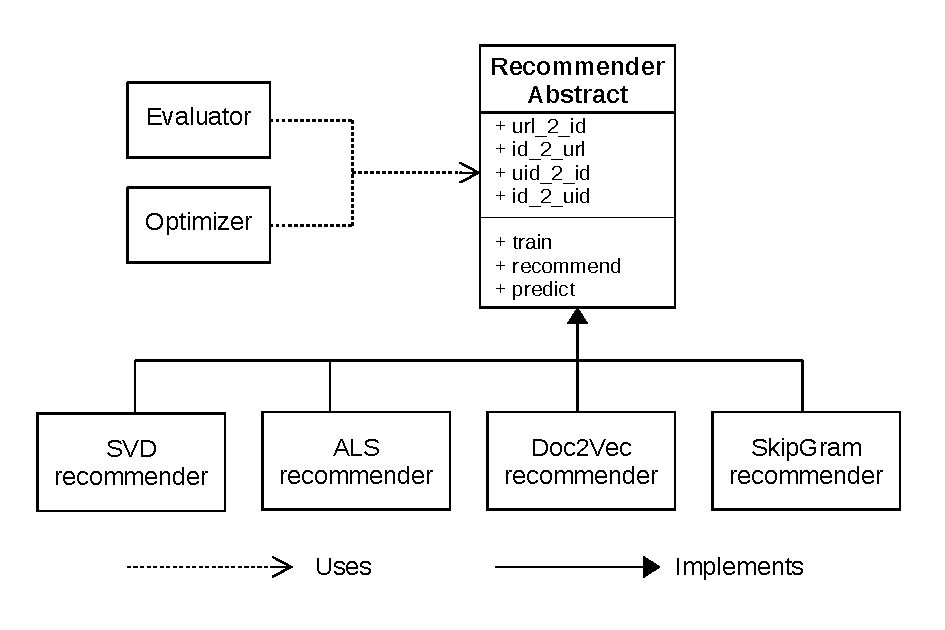
\includegraphics[scale=0.9]{obrazky-figures/class_diagram.pdf}
    \caption{Class diagram showing the hierarchy of the created models.}
    \label{fig:class_diagram}
\end{figure}

\subsection*{RecommenderAbstract}
An abstract class that all the other recommender models have to inherit from. It defines the following properties:

\begin{itemize}
    \item \texttt{url\_2\_id}: A dictionary mapping URLs of pages to model specific unique identifiers, used for indexing within the model. 
    \item \texttt{id\_2\_url}: Dictionary mapping model specific IDs back to URLs.

    \item \texttt{uid\_2\_id}: Dictionary mapping user identifiers used in the dataset, to model specific unique IDs.

    \item \texttt{id\_2\_uid}: Dictionary mapping model specific IDs back to user identifiers used in the dataset.

\end{itemize}
Alongside with the above properties, the class also defines a couple of methods, that the inherited classes have to implement:
\begin{itemize}
    \item \texttt{train(*parameters)}: The method used to invoke training of the model. The number of parameters is variable and model specific. These are usually the hyperparameters, such as the number of epochs, learning rate etc. 
    
    \item \texttt{predict(uid, url)}: This method can be called to predict the score for a user, specified by the uid parameter, and an item, specified by its url. The returned score is an indicator of how suitable is this item for the specified user.
    
    \item \texttt{recommend(uid, n)}: Returns an ordered list of top n recommendations for a user, specified by his user ID (uid).
\end{itemize}

\subsection*{Evaluator}
The Evaluator class was created with the intention of having a simple and fast way of evaluating the recommender models. Hence for, it was constructed to work with the AbstractRecommender class. To create the Evaluator, an already trained recommender model has to be passed to the initialization method. From then the evaluator works with this exact model. Consequently, the model can be evaluated by simply calling one of the methods implemented in the Evaluator class. The class implements the following methods:

\begin{itemize}
    \item \texttt{rank\_evaluation(test\_set)}: Evaluates the model on the given test\_set using the RANK metric. The \texttt{test\_set} parameter has to be a pandas DataFrame object and can be created using a function called \texttt{train\_test\_df}.
    
    \item \texttt{recall\_at\_k(test\_set, k)}: Evaluates the model on the given test set using the recall at k metric. This metric looks at how many of the items from the test set occur in the top \texttt{k} created recommendations.
    
    \item \texttt{precision\_at\_evaluation(test\_set, k)}: Evaluates the model using the precision at k metric. This metric looks at how many of the items from the test set occur in the top k created recommendations.
    
    \item \texttt{mse(test\_set)}: Evaluates the model by computing the mean square error between the computed scores and the actual values of interactions. This metric only makes sense for the SVD and ALS models, as they create an interaction matrix. 
\end{itemize}
More on the topic of evaluation, together with the description of the above-mentioned evaluation metrics, can be found in section \ref{evaluation}.

\subsection*{Optimizer}
The Optimizer class is used for tuning the models by finding the optimal hyperparameters. It does so, for it repeatedly trains the model and evaluates it using the Evaluator class. The optimal parameters are those that achieve the best results during evaluation. 

The number of parameters, together with their exact purpose, is model specific. Therefore the Optimizer class is designed to work with the abstract recommender class, which allows it to create a uniform way of usage, no matter the specific model it is optimizing. Once again the model to be optimized is passed as a parameter to the initialization method, together with a list of parameters and a search space.

The list of parameters has to contain the exact names of parameters defined in the \texttt{train} method of the model in concern. The last parameter defines a search space for each one of the parameters in the list. A search space can be defined simply as a range of values, or as a probabilistic distribution from which the values are going to be sampled. 

After the optimizer has been initialized, everything is ready for the optimization itself to start. The most straightforward method for optimization is a simple grid search. Here the model is simply evaluated with all the possible combinations of the parameter values. That, however, makes it very time consuming and therefore rather impractical. An improvement to this problem comes with random search approaches, that sample the values randomly from the given parameter space. These approaches are faster than grid search however do not offer the same guarantee of finding the optimum. Other popular methods use techniques like decision trees and various Bayesian approaches. The optimizer class offers the following methods:
\begin{itemize}
    \item \texttt{optimize\_forest}: This method uses the forest\_minimize function - from the \texttt{skopt} library - to optimize the model. This function implements a decision tree regression search, that sequentially evaluates the model at the next best point. 
    
    \item \texttt{optimize\_hyperopt}: This method uses the \texttt{Hyperopt} library, that applies Bayesian approaches for finding the optimal parameters. This particular method works with the Tree of Parzen Estimators (TPE) algorithm, that attempts to approximate the performance of hyperparameters, based on already completed measurements. This algorithm seemed to serve better for our models as it reached the optimum in fewer steps.
\end{itemize}
Both of these methods require the following parameters:
\begin{itemize}
    \item train: The dataset on which the model will be trained.
    \item test: The dataset used for evaluation.
    \item metric: Defines the evaluation technique that will be used in the Evaluator class. The default value is set to ‘rank’, meaning the RANK evaluation technique. Other options are ’recall’ and ’precision’.
\end{itemize}



%===============================================
% User Mappings
%===============================================
\section{User Mappings} \label{user_mappings}
The mechanism strives to combine both \texttt{user\_id} and \texttt{visitor\_id} to create a unique user identifier. Here, when processing interactions, the system works as follows:

\begin{itemize}
    \item In an interaction with no \texttt{user\_id}, the user is represented only with the \texttt{visitor\_id}.
    
    \item In an interaction with both \texttt{visitor\_id} and \texttt{user\_id}, the user is represented with the \texttt{user\_id} and the system remembers that the \texttt{visitor\_id} was used together with it. 
\end{itemize}
Applying these two approaches brings the system numerous advantages:

\begin{enumerate}
    \item It is able to connect interactions, where only the \texttt{visitor\_id} is known, to the actual user, once he is logged in and creates new interactions with his \texttt{user\_id}.

    \item It can represent users both by their \texttt{visitor\_id} or their \texttt{user\_id} individually but also link them together. That means when a user created some interactions with his \texttt{user\_id} and than logged out but still had the same \texttt{visitor\_id}, the system is able to identify him.

    \item It handles cases where one \texttt{user\_id} is used with more \texttt{visitor\_ids}. These cases occur when people use multiple browsers or multiple computers. The class stores a list with all \texttt{visitor\_ids} that were used together with the \texttt{user\_id}.

    \item It handles cases where one \texttt{visitor\_id} is used with more than one \texttt{user\_id}. In these cases, multiple users logged in on the same computer. Here interactions, where only the \texttt{visitor\_id} is known, cannot be used on their own because the system is not able to distinguish what user should it assign them to.
\end{enumerate}
By applying this class to identify the users the dataset remained much bigger than when only the \texttt{user\_id} was used. From the original 265123 interactions, only 655 were lost, because the system was not able to identify the users. That means about 99.75\% of the dataset has remained. Compared to the 29\% of \texttt{user\_ids} it is a big improvement. The~results of comparing those two approaches are shown in table \ref{tab:dataset_comparison}. \\ \\


\begin{table}[h!]
    \centering
    \begin{tabular}{@{}lccc@{}}
    \toprule
                           & \textbf{original dataset} & \cellcolor[HTML]{A4C2F4}\textbf{user\_id} & \cellcolor[HTML]{FFCCC9}\textbf{UserMappings} \\ \midrule
    \rowcolor[HTML]{EFEFEF} 
    num of interactions    & 265 123                   & 76 369 (29\%)                             & 264 468 (99.75\%)                               \\
    num of users           & -                         & 36 412                                    & 175 794                                         \\
    \rowcolor[HTML]{EFEFEF} 
    num of pages           & 2187                      & 1642                                      & 1996                                            \\
    average pages per user & -                         & 1.9                                       & 1.4                                             \\
    \rowcolor[HTML]{EFEFEF} 
    average users per page & -                         & 41                                        & 123                                             \\
    sparsity               & -                         & 99.87\%                                   & 99.92\%                                         \\
    \rowcolor[HTML]{EFEFEF} 
    interactions per day   & 1473                      & 424                                       & 1469                                            \\ \bottomrule
    \end{tabular}
    \caption{The first column shows the original dataset, the second shows the dataset when only \texttt{user\_id} is used to identify users and the last shows the results of applying the \texttt{UserMappings} method. When using only the \texttt{user\_ids} only 29\% of the dataset remained, whereas when using user mappings this number reaches to 99.75\%. The number of users, average pages per user and average users per page in the original dataset cannot be computed.}
    \label{tab:dataset_comparison}
\end{table}

The results of the above comparison show us some advantages of both approaches, to~name a few:
\begin{itemize}
\item Applying user mappings preserves significantly more from the original dataset.
\item With using only \texttt{user\_ids} the sparsity of the resulting dataset is lower.
\item \texttt{User\_ids} result in bigger average number of pages per user.
\end{itemize}
The conclusion of the comparison is that when only \texttt{user\_ids} are used the resulting dataset is denser and hence the dataset should be more valuable for the recommendation problem. On the other hand, applying user mappings preserves much more data. In fact, the cause of user mappings having a lower average of pages per user is that the dataset contains more users that have only one interaction. Such users are not very useful to the recommender system. 

In fact, about 79\% of users, created with \texttt{UserMappings}, visited only one webpage. These users produced nearly 55\% of all interactions in the dataset. In the \texttt{user\_id} dataset the numbers are lower with only 66\% of users having just 1 unique interaction, and formulating 33\% of the dataset. The number of unique interactions per user is critical to the performance of the recommender. It is natural that as the number grows the number~of users decreases exponentially, as shown in figure \ref{uid_3_pages}.


\begin{figure}[H]
    \centering
    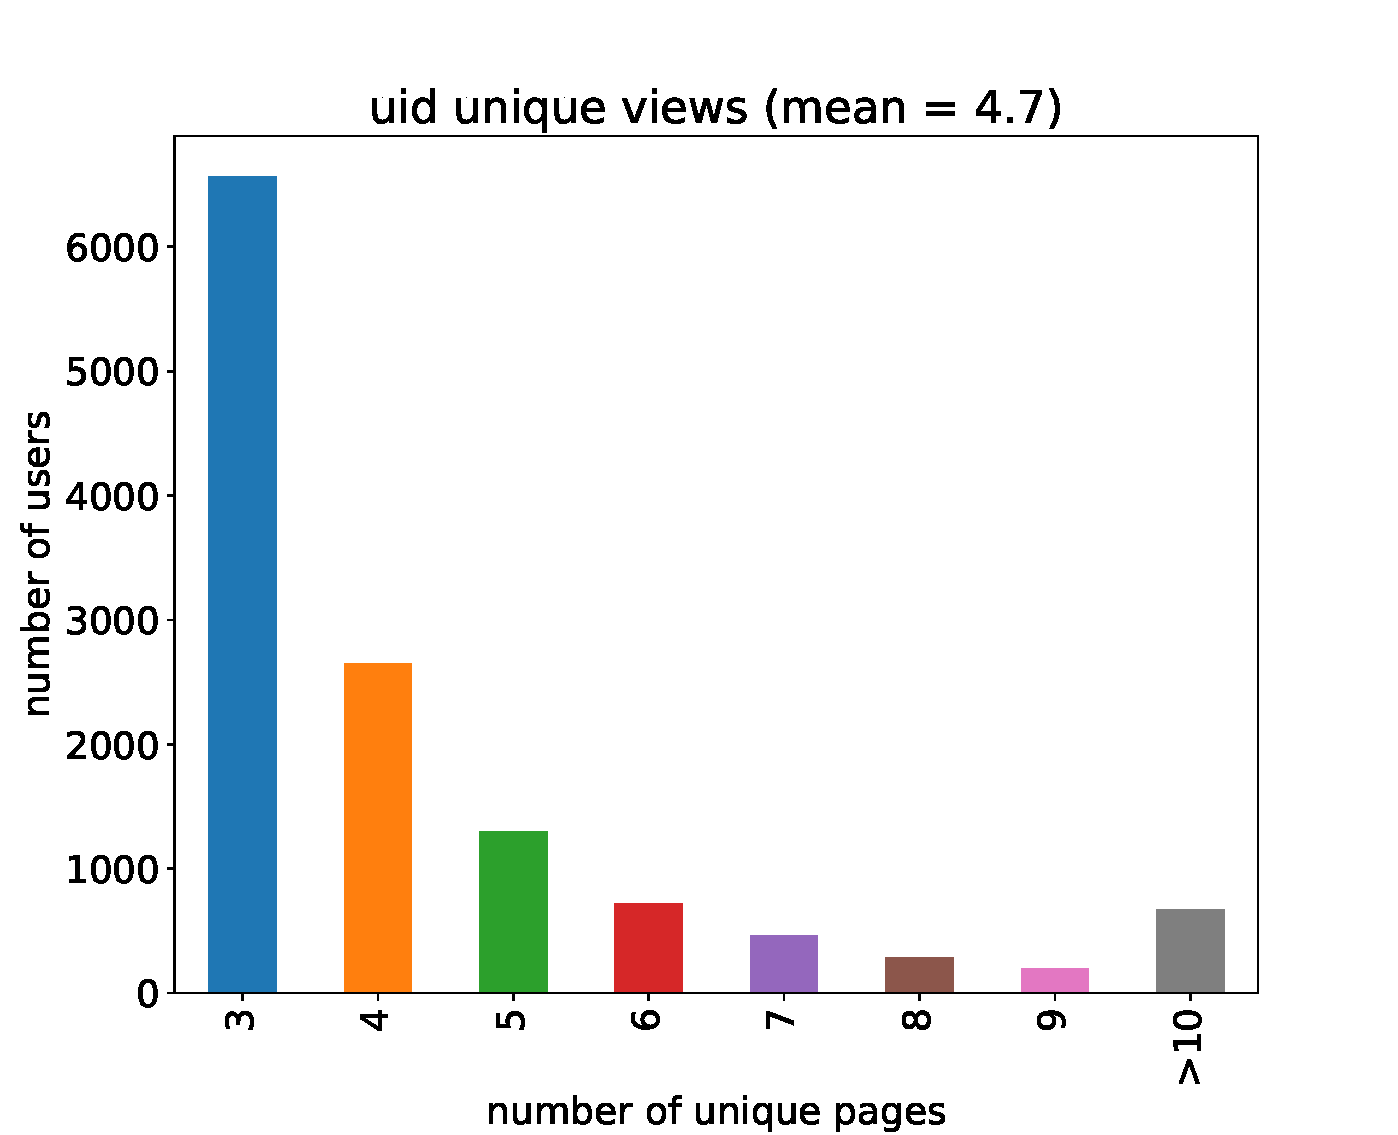
\includegraphics[scale=0.5]{obrazky-figures/uid_3_pages.pdf}
    \caption{This graph shows the number of users according to the number of unique webpages they visited. It shows, for example, that nearly 7000 users visited exactly 3 pages, nearly 3000 users visited exactly 4 unique pages etc.}
    \label{uid_3_pages}
\end{figure}

\begin{figure}[H]
\centering
\begin{subfigure}{.5\textwidth}
  \centering
  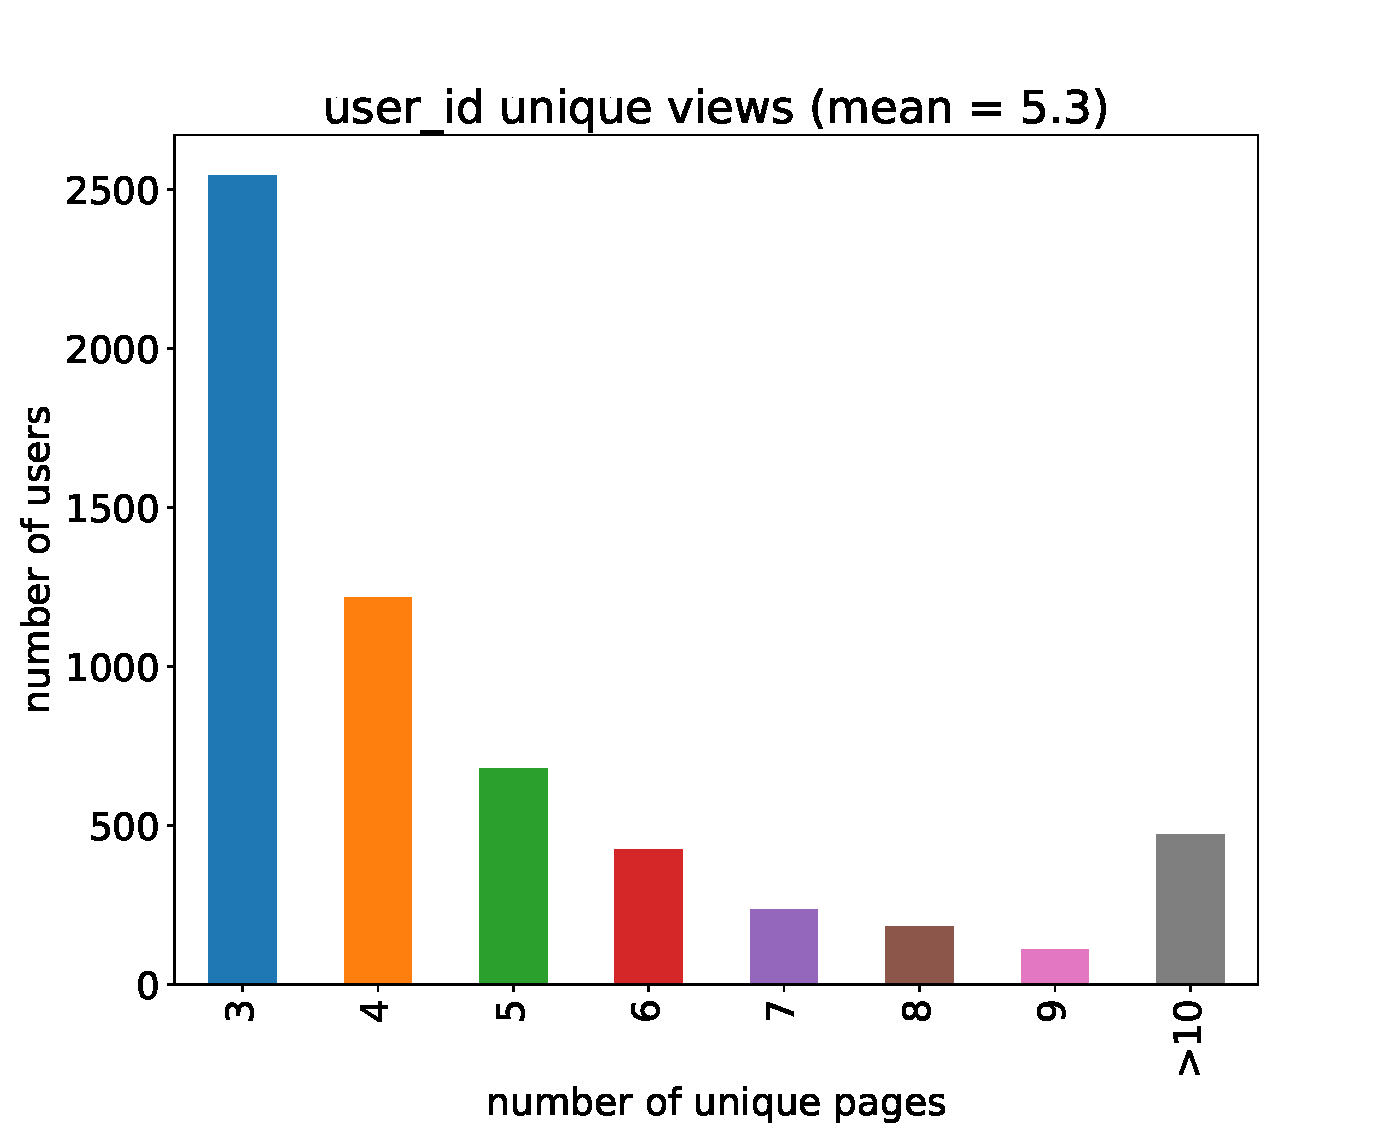
\includegraphics[scale=0.34]{obrazky-figures/user_3_pages.pdf}
  \caption{user\_id}
  \label{fig:unique_pages_comparison_user_id}
\end{subfigure}%
\begin{subfigure}{.5\textwidth}
  \centering
  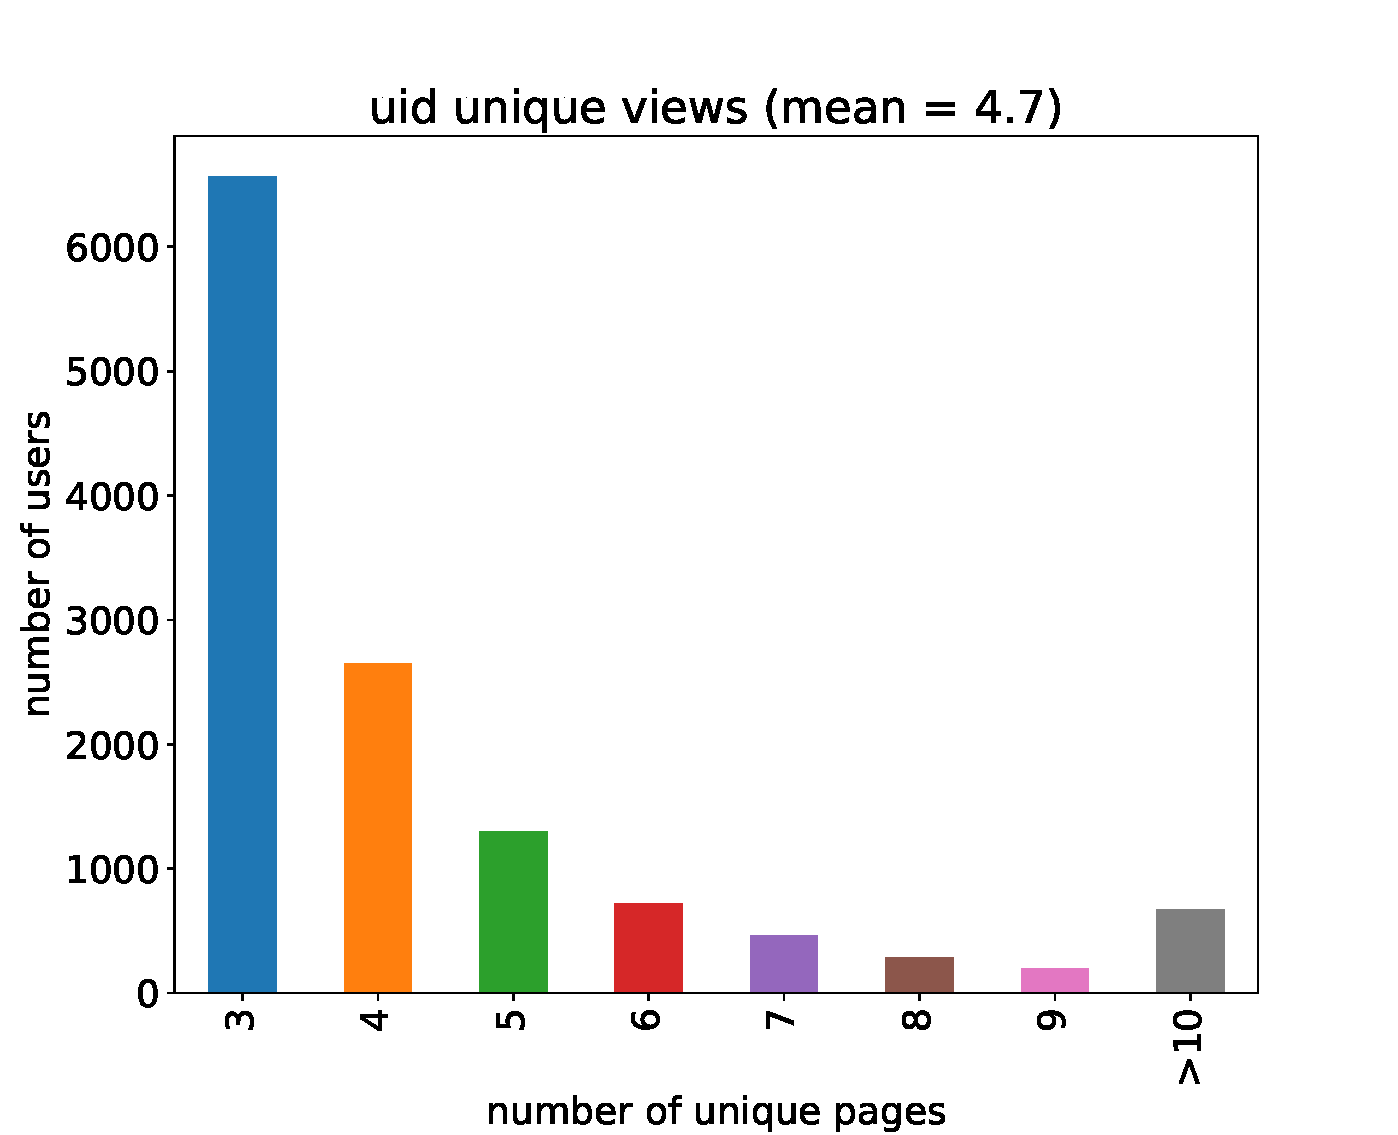
\includegraphics[scale=0.34]{obrazky-figures/uid_3_pages.pdf}
  \caption{UserMappings}
  \label{fig:unique_pages_comparison_uid}
\end{subfigure}
\caption{Comparison of \texttt{user\_id} and \texttt{UserMappings} datasets. The graphs show the number of users according to the number of unique webpages that they visited.}
\label{fig:unique_pages_comparison}
\end{figure}

Both \texttt{UserMappings} and \texttt{user\_id} approaches generate a nearly identical shape of the decrease. It is worth noting though, that \texttt{UserMappings} generate much bigger numbers. As already mentioned it contains more users who have only one unique interaction. However, it also contains more users that have a significant number of interactions, users that have big informational value to the system. 

With \texttt{UserMappings}, the dataset contains 1535 more users, who have at least 5 unique interactions, than the \texttt{user\_ids} dataset and 198 more users with 10 and more interactions. These users have an important role for the recommender and getting rid of them would be a significant loss. A side by side comparison of dataset sizes changing with the minimum number of interactions per user is visualized in figure \ref{side_by_size}.

\begin{figure}[H]
    \centering
    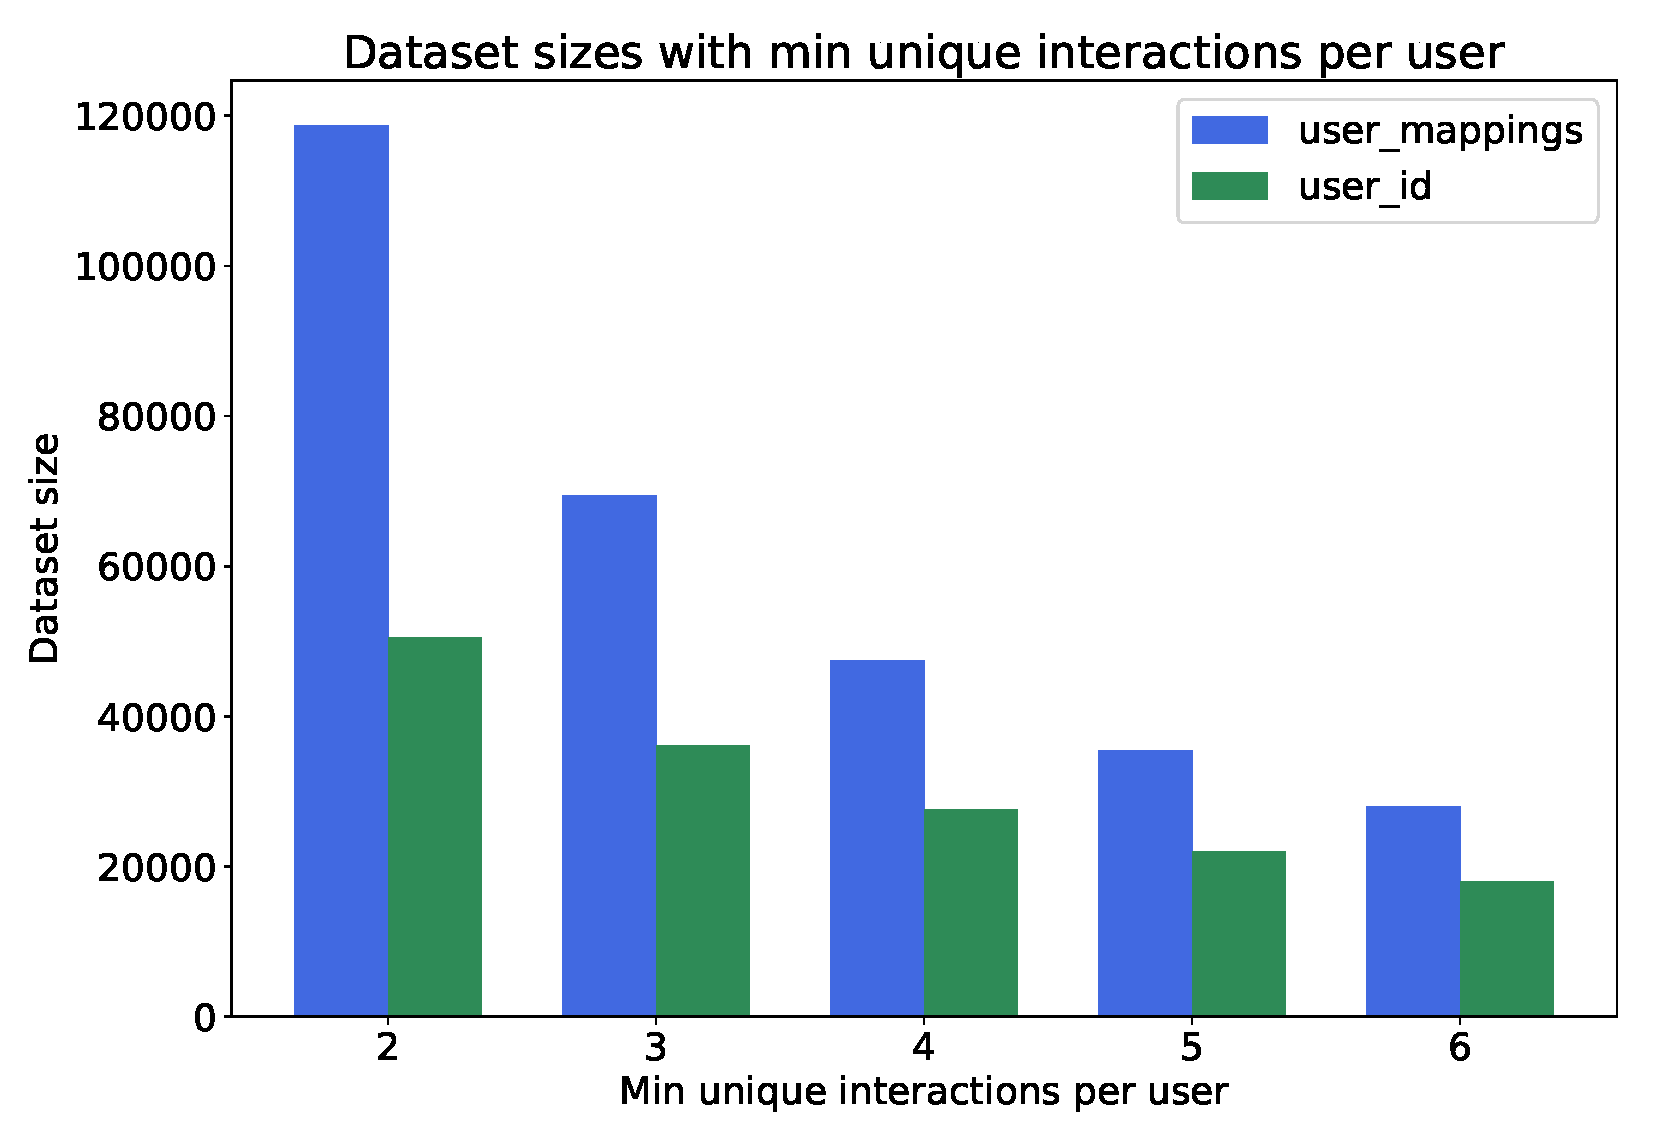
\includegraphics[scale=0.5]{obrazky-figures/min_interaction_sizes.pdf}
    \caption{A side by side comparison of dataset sizes according to the minimum number of interactions per user. The first two columns, for example, show the dataset sizes with having only users that interacted at least with 2 (x-axis) different pages etc.}
    \label{side_by_size}
\end{figure}

The system may even work only with users with 5 or more interactions and in those cases, the size of the dataset would be crucial. Moreover, the number of unique users per page is also much bigger with \texttt{UserMappings}, as shown in figure \ref{fig:page_views_comparison}.

All these factors suggested that the mechanism of \texttt{UserMappings} should be more beneficial for the system and led to the decision of using them instead of the original \texttt{user\_ids}.

\begin{figure}[H]
\centering
\begin{subfigure}{.5\textwidth}
  \centering
  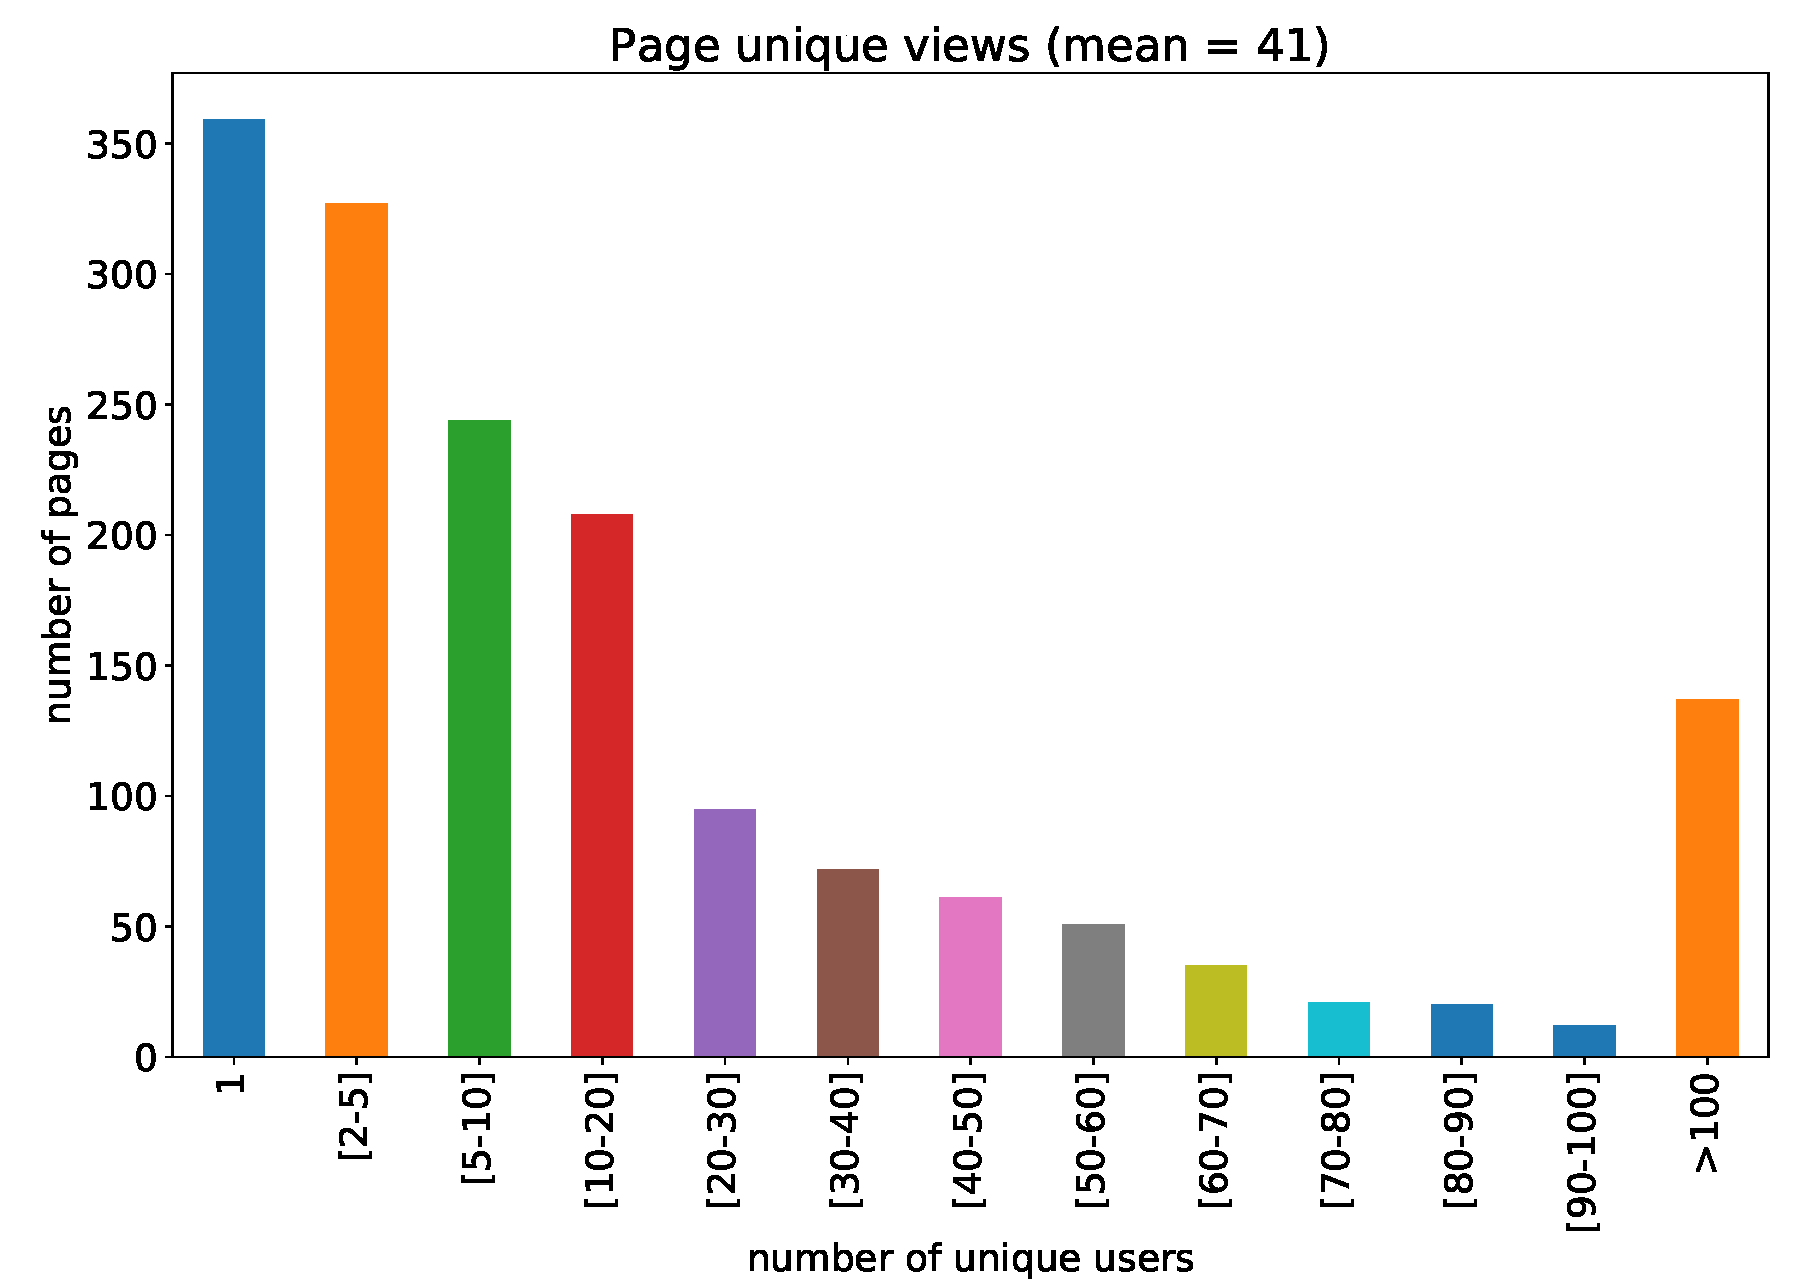
\includegraphics[width=1.\linewidth]{obrazky-figures/page_unique_users.pdf}
  \caption{user\_id}
  \label{fig:page_views_comparison_user_id}
\end{subfigure}%
\begin{subfigure}{.5\textwidth}
  \centering
  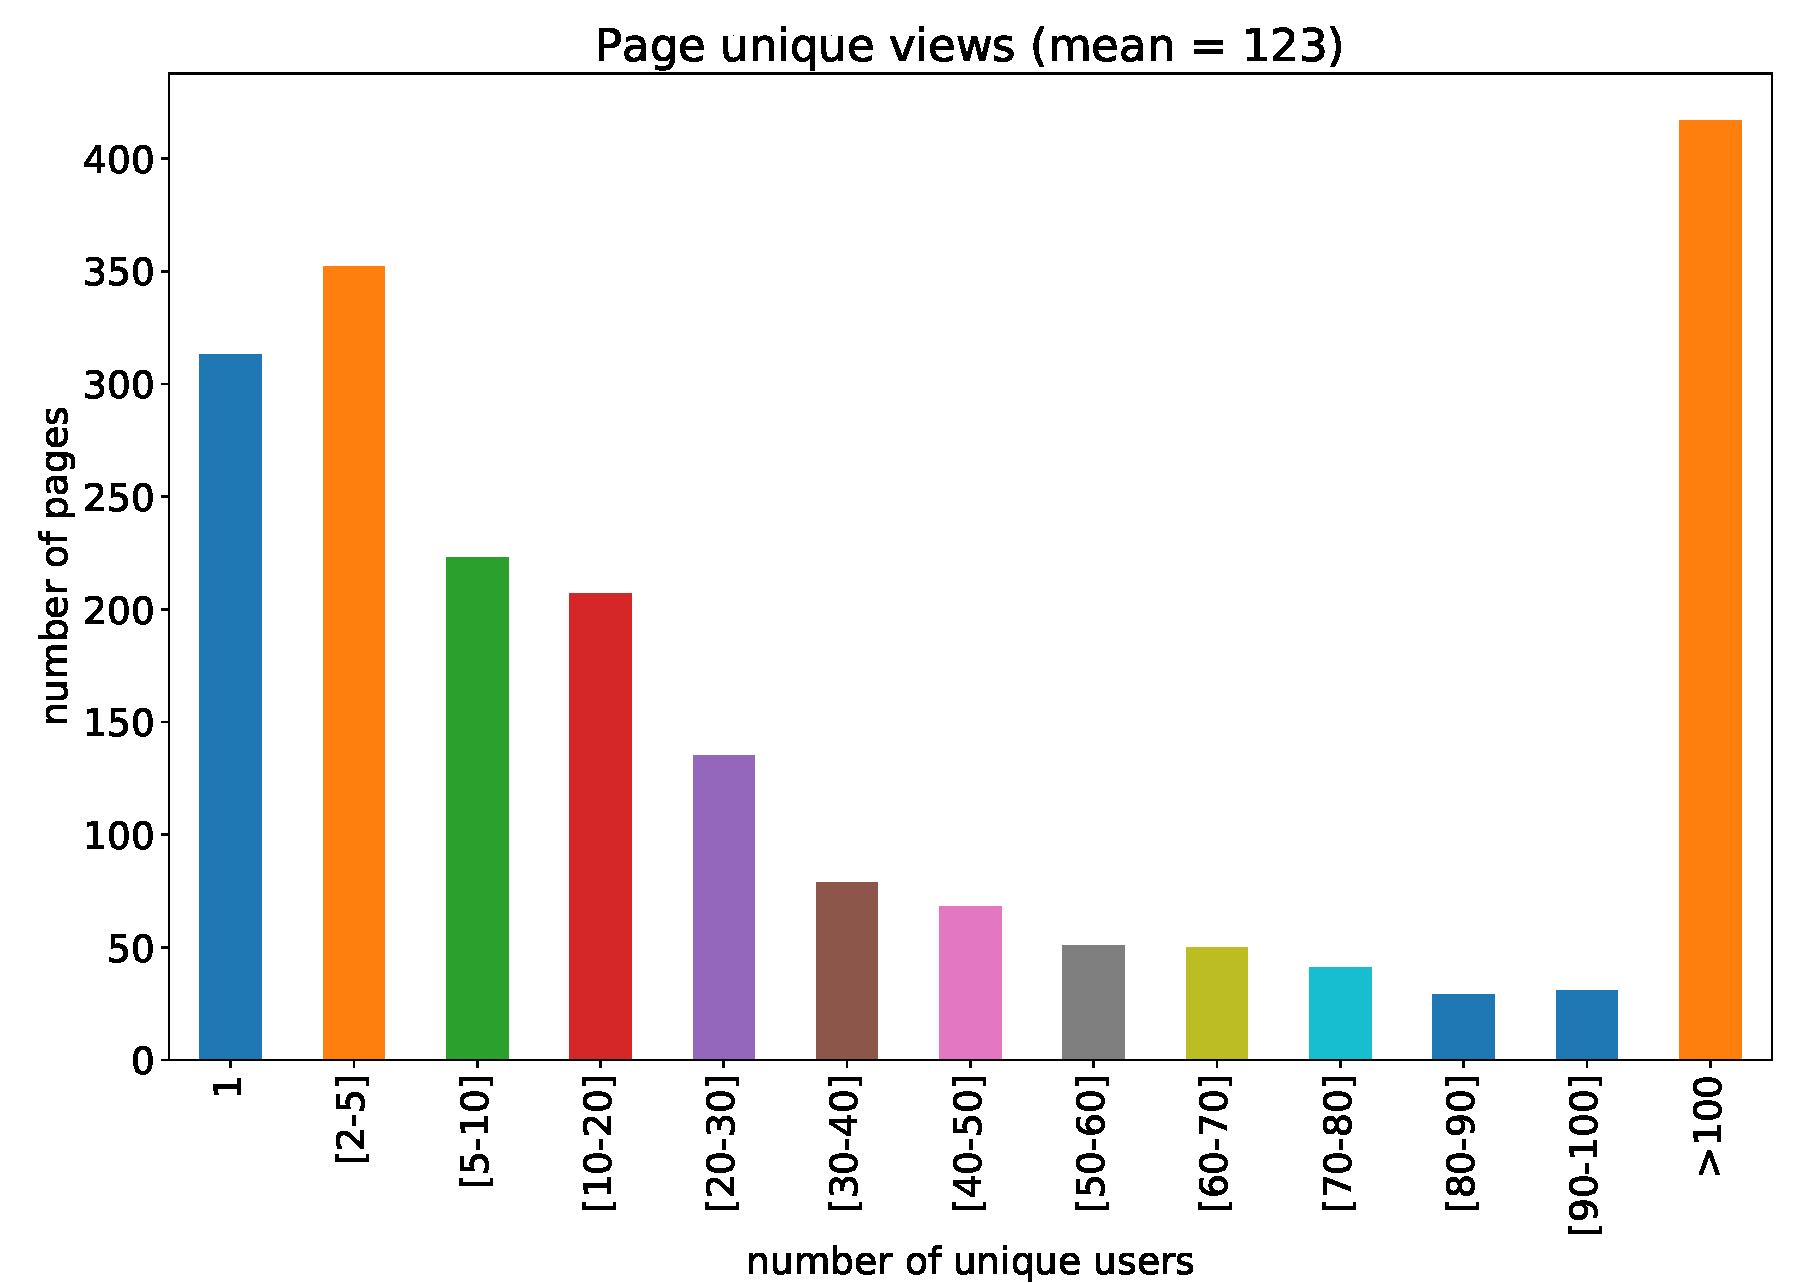
\includegraphics[width=1.\linewidth]{obrazky-figures/page_unique_uid.pdf}
  \caption{UserMappings}
  \label{fig:page_views_comparison_uid}
\end{subfigure}
\caption{A comparison of page visits. The x-axis shows the number of unique visits on a~page, the y-axis shows the number of pages. With \texttt{UserMappings}, for example, around 350 pages were visited only by 2-5 unique users etc.}
\label{fig:page_views_comparison}
\end{figure}



%===============================================
% Section
%===============================================
\section{SVD recommender} \label{svd_implementation}
The first model to discuss is the \texttt{SVDModel} class. This approach is based on singular value decomposition, a technique already described in \ref{latent_factor_models}. To remind of its application, it first creates a matrix of user-item interactions. To do so, it uses the \texttt{make\_sparse} method. 

\subsection*{Creating the interaction matrix}
To construct a sparse matrix of user-item interactions a function called \texttt{make\_sparse} was created. This function creates an object of class \texttt{IncrementalSparseMatrix} (ISM), that is able to hold the interactions in essential data types as lists and dictionaries. The \texttt{make\_sparse} function then iterates over the rows of the dataset, each time adding one interaction to the ISM object, using the \texttt{add(row, col, data)} method. The row and col parameters determine the row and column in the matrix, that actually represent a particular user and item. The data parameter is the numeric value of the interaction, being the time spent on the webpage of an article. \\ \\
After all the interactions have been added, the ISM object can create the sparse matrix from its interactions, by calling a method called \texttt{to\_coo}. This method returns a \texttt{sparse\_coo} object, defined in scipy.sparse module. The final values in the \texttt{sparse\_coo} matrix, however,  are not going to be the time passed to the add method. They are computed from the time values using one of the implemented metrics, transforming the time into confidence levels, as described in section \ref{implicit_datasets}. 
The \texttt{to\_coo} method of the ISM class enables to choose the used metric, by specifying it in the metric parameter. This parameter can receive the following values:
\begin{itemize}
    \item \texttt{log}: Applies equation \ref{eq:log_conf} to compute the confidence from the numeric value of each interaction, being the time.
    \item \texttt{lin}: Computes the confidence using equation \ref{eq:lin_conf}.
    \item \texttt{bin}: Here the numeric value of an interaction is simply binarized. That means the resulting \texttt{sparse\_coo} matrix will only consist of zeros and ones, indicating whether the particular interaction occurred or not.
\end{itemize}
After the creation of the \texttt{sparse\_coo} matrix, it is passed to the \texttt{svd} function from the \texttt{numpy.linalg} module. This function performs the decomposition and returns the three created matrices $U$, $S$, $V$. Where $U$ represents the latent features of users, $V$ represents features of items and $S$ is a diagonal matrix giving the relative significance of these factors. 

At that moment the model is ready to start creating recommendations. The prediction of preference is simply done by taking the dot product of corresponding vectors from $U$ and $V$. Put into practice, the interaction of user $u$ and item $i$ would be computed as:
\begin{equation}
    r_{ui} = U_u V_i
\end{equation}
To recommend user $u$ the top $n$ items, the model simply multiplies the $U_u$ vector with the whole $V$ matrix, sorts the values in descending order and returns the first $n$ items.

%===============================================
% Section
%===============================================
\section{ALS recommender} \label{als_implementation}
The next model to describe is the \texttt{ImplicitALS} class. This model is an example of a traditional collaborative filtering technique on an implicit dataset, using matrix factorization. Matrix factorization techniques were already presented in section \ref{cf_theory}. Similarly to the model using SVD, first of all, the interaction matrix has to be constructed. Several experiments with varying confidence values were performed and are summed up in detail in section \ref{evaluation}. 

Then the interaction matrix is passed to \texttt{AlternatingLeastSquare} function from the \texttt{implicit.als} library created by Ben Frederickson \cite{BenImplicit}. The models in this library are written in Cython and even can fit the data on a GPU. That makes them very attractive to use as they are really fast and efficient. This method performs the factorization of the interaction matrix, decomposing it into two separate matrices, which when multiplied together result in an approximation of the original matrix. For finding the right values in these matrices and hence for actually training the model, the Alternating least squares (ALS) algorithm is used. The \texttt{implicit.als} module implements the exact ALS model defined in paper \cite{Implicit}. 

After the training, the retrieved matrices are stored in two attributes of the \texttt{ImplicitALS} class. The \texttt{user\_factors} attribute stores the matrix representing vectors of users and the \texttt{item\_factors} attribute holds the matrix of item vectors. The prediction, as well as the recommendation, is done the exact same way as in the SVD model. That is, by simply taking the dot product of the corresponding vectors. This technique represents one of the most common techniques used for the task of recommendations. It also showed to perform very well in our case.

%===============================================
% Section
%===============================================
\section{Doc2Vec recommender} \label{doc2vec_implementation}
The next model to discuss is implemented in \texttt{Doc2VecModel} class. This model is an example of a content-based recommender, where the recommendations are based only on the content of its items. In this particular case, the items are web articles and their content is therefore textual. It is stored in a JSON file together with the rest of the obtained additional information. To create representations that are capable of modelling similarities, the Doc2Vec model was used. In particular its implementation in the \texttt{gensim} library. This approach not only enables the model to learn document vectors during the training, but it also makes it possible to infer vectors of new unseen documents after the model has been already trained. It does so by creating a paragraph vector for the new document and training this paragraph vector until convergence while the already trained word vectors are fixed.

To be able to pass the obtained textual content data, that contain the title and the first paragraph of an article, to the Doc2Vec model, it has to be first pre-processed. The \texttt{gensim} library limits the doc2vec model to work with objects of \texttt{TaggedDocument} class. Objects of this class contain a list that holds the text of one document split by words, while preserving their order,  and a number identifying the corresponding document. In the concern of providing an easy and fast way of pre-processing the data, the \texttt{Doc2VecInput} class was created. First, the JSON file, that contains all the obtained metadata, has to be loaded into a dictionary. Then this dictionary is simply passed to the \texttt{Doc2VecInput} class, that creates \texttt{TaggedDocument} objects for all items and stores them into a list being the appropriate input to the actual doc2vec model.

The created input is then passed to an object of the \texttt{Doc2VecModel} class, together with the data set containing the user-item interactions. This class implements a wrapper of the original Doc2Vec model from the \texttt{gensim} library. Once the object is constructed, it can either train the model only on the given input documents or use an already pre-trained model, containing 300-dimensional vectors, trained using the DBOW model on English Wikipedia pages, to only infer the vectors for the input documents. To actually train the model, the \texttt{train} method is used. To retrieve the pre-trained model and only infer the given documents into vectors, the \texttt{load\_pretrained} method should be used. 

After that, the created vectors are stored in the \texttt{doc\_vectors} property. At that point, it is possible to use these vectors to compute similarities between items. To perform the actual recommendation though, the model first has to create vectors for its users.

\subsection*{Creating user vectors}
All users are described by the items they interacted with. The representation of users is hence created directly using their item vectors, that have already been pre-trained. There~are several ways of transforming the item vectors to create a representation for a user. The \texttt{Doc2VecModel} class implements the following two methods, each taking a slightly different path.

\begin{itemize}
    \item \texttt{create\_user\_vectors\_log(alpha, epsilon)}: In this method, users are represented as a weighted arithmetic mean of their item vectors. The weights are actually the confidence values computed applying the logarithmic confidence metric \ref{eq:log_conf}. That also explains the necessity of the alpha and epsilon parameters, as they are needed for computing the confidence in this metric.
    
    \item \texttt{create\_user\_vectors\_bin()}: As opposed to the first-mentioned method, here users are represented only as a sum of their item vectors. Therefore this method does not require any additional parameters.
\end{itemize}
In the beginning, these methods were constructed using two for cycles, iterating over all users and all their items. This approach pretty obviously turned out to be very slow. Hence for it was later on optimized to use matrix factorization in numpy. When the sparse matrix, containing confidence values, is multiplied by the matrix of document vectors, the resulting matrix will contain the desired user vectors.

\begin{figure}[H]
    \centering
    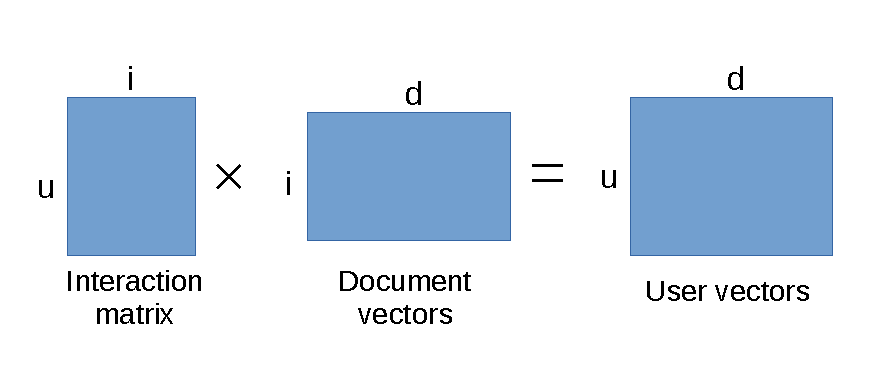
\includegraphics{obrazky-figures/user_vectors.pdf}
    \caption{Shows the creation of user vectors, by multiplying the sparse interaction matrix with the matrix containing document vectors. Here, $u$ is the number of users, $i$ is the number of items and $d$ is the dimensionality of document vectors.}
\end{figure}

After computing the user vectors, the model is ready to start recommending. The~process of creating both predictions and recommendations once again consists only of taking the dot product of corresponding user and item vectors.

%===============================================
% Section
%===============================================
\section{Skip-gram recommender} \label{skipgram_implementation}
The last model that will be explained is the Skip-gram recommender, that implements the already discussed approach, based on the skip-gram negative sampling model, described in section \ref{proposed}. It is implemented in \texttt{SkipGramModel} and \texttt{SkipGramRecommender} classes and uses an open source deep learning platform called \texttt{pytorch}.
This library defines a way of constructing a neural network, by inheriting from its \texttt{nn.module} class. The neural network architecture itself is implemented within the \texttt{SkipGramModel} class, that inherits from the \texttt{nn.module}. It first creates and initializes all the needed parameters, it stores the document vectors, that are passed to the model already pre-trained and are fixed during the training, initializes embeddings for tags that, on the other hand, are going to be learned during the training and creates two linear layers with one rectified linear unit (ReLU) and \texttt{nn.LogSigmoid} class for applying element-wise logarithm of the sigmoid function.

All classes that inherit from the \texttt{nn.module} have to override the \texttt{forward} function, that represents a single step of the computation. This function is repeatedly called during the training process, each time returning the computed loss. The \texttt{SkipGramModel} class defines the forward function as:
\begin{itemize}
    \item \texttt{forward(item\_batch, context\_batch, neg\_batch)}
\end{itemize}
Where \texttt{item\_batch} contains a list of batch\_size item identifiers. The \texttt{context\_batch} is a list of batch\_size users that each interacted with the corresponding item from \texttt{item\_batch}. However, this list does not contain user IDs. Users are created from items they have interacted with. Therefore, instead of an ID, users are represented as lists of item IDs and the \texttt{context\_batch} is a list of lists containing item IDs. Similarly the \texttt{neg\_batch} contains a list of negative samples for each item in the \texttt{item\_batch}. A negative sample of an item is actually a user that has not interacted with it. The user is once again represented as a~list of its item IDs. 

The \texttt{forward} function first constructs item and user vectors from the passed batches, using their tag embeddings and document vectors. Then it sends these vectors into the network to create item and user embeddings. Finally, these embeddings are used to compute the loss value, defined by function \ref{eq:skip-gram} and \ref{eq:neg_sampling}. The transformation of an item vector into an embedding is visualized in figure \ref{fig:layers}.

\begin{figure}[H]
    \centering
    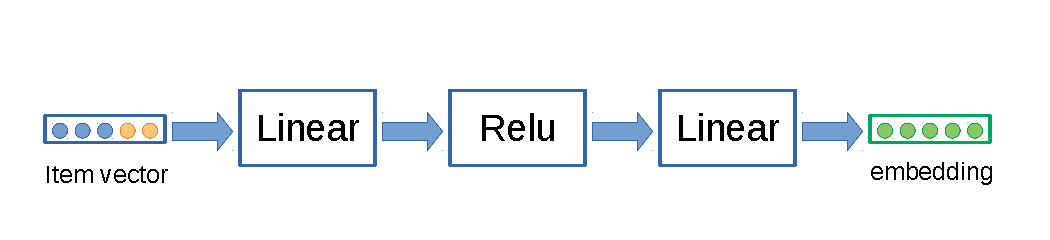
\includegraphics[scale=0.9]{obrazky-figures/layers.pdf}
    \caption{Shows the creation of item embeddings. The item vector, consisting of its tag embeddings concatenated with its document vector, is sent to the neural network that consists of two linear layers with one rectified linear unit (ReLU).}
    \label{fig:layers}
\end{figure}

The \texttt{SkipGramRecommender} class is used to create an actual recommender system from the neural network architecture implemented in the \texttt{SkipGramModel}. That means it inherits from the RecommenderAbstract class and implements all the required methods. The most important of which is the \texttt{train} method. 

In this method, the actual training of the network is performed. First, it needs to prepare all the needed components for the execution of the training, like the \texttt{SkipGramModel}, a~data pipeline for generating the batches and an optimizer object from the \texttt{torch.optim} module. The \texttt{Adam} optimizer was used in this case. After all the preparation is completed the training can start. The \texttt{train} method is provided with a parameter that defines the number of epochs. In each epoch, a new batch generator is created. Then this generator is iterated, each time generating a new batch, that is passed to the \texttt{forward} method of the network. This method processes the given batch and returns the computed loss. After that the model calculates the gradients and backpropagates them to adjust all its parameters, being weights of its linear layers and the tag embeddings. 

After iterating over all epochs the training process is finished and the recommender is ready to perform. 



%===============================================
% Evaluation
%===============================================
\chapter{Evaluation} \label{evaluation}
This section provides insights into the process of evaluating the implemented recommenders. Evaluation of recommender systems - and in particular recommender systems working with implicit feedback - is by itself, a very challenging problem. It is important to realize, that these datasets do not provide a reliable source of feedback regarding which items users do not like, as not interacting with an item should not be interpreted as not liking it. Also, it is important to note that our system does not have the ability to track reactions of users to their created recommendations, as it is commonly implemented in production. Therefore the system can only be evaluated offline, by splitting the dataset into two separate parts, one used to train the model and the other to evaluate its performance by looking at the computed ranking of the actual interactions that the model was not trained on. 

Refer to chapter \ref{eval_metrics} that explained the theory behind the three evaluation metrics used in this thesis. First, section \ref{eval_experiments} starts by reviewing the performed experiments, briefly touches the topic of the ablation study and describes the evaluation set-up together with the process of splitting the original dataset into two separate sets for training and evaluation. Finally, section \ref{eval_results} reveals the results of all three evaluation metrics applied to the implemented recommenders and closes with a discussion on their effectiveness and usefulness.



\section{Performed experiments} \label{eval_experiments}
This section offers a brief summary of the experiments that were performed with the recommendation models. All models were trained and evaluated on two separate datasets, that were created using the \texttt{train\_test\_df} function. The minimal number of interactions for a user, to be included in the test set, was set to 6. By that, the system evaluates the models only on users that interacted with at least 3 different pages. 

\subsection*{Creating the test set}
Two separate datasets were used for training and evaluating the recommenders. A function called \texttt{train\_test\_df} was created to provide a convenient way of splitting the original dataset into a training set and a test set. It is worth considering a couple of things before creating a test set for a recommender system. 

First, the system can only deal with existing users and items it is aware of and hence contains a vector representation for them. That means that the set of users and the set of items, in the training and test datasets, have to equal. Second, it is only reasonable to evaluate on users that have at least a certain number of interactions, as users with only one interaction do not provide enough data to receive any valuable recommendations. The~\texttt{train\_test\_df} is defined as follows:

\begin{itemize}
    \item \texttt{train\_test\_df(df, min\_interactions)}: this function splits the original dataset, being the df parameter, and returns the created training and test datasets. The \texttt{min\_interactions} parameter defines the minimum required number of unique interactions for a user to be included in the test set. Two interactions of a user are unique if they were created with two different items. If a user has more interactions than that, they are split in half. The first half goes to the training dataset and the second half to the test dataset.
\end{itemize}

This function split the original dataset into a training set containing 250 661 interactions and a test set with 13~807 interactions. The test set was used to find optimal hyperparameters of the models during optimization. After finding the optimal hyperparameters all models were evaluated again, this time using a validation set. As described in section \ref{our_dataset}, the original dataset used in this thesis consists of records collected over six months (from September 2018 to February 2019). The validation set contains interactions created in the two following months (March and April 2019). It includes a total of 17 658 interactions, 7363 unique user Ids and 1143 page URLs. 

The first experiment was based on trying different confidence values in the interaction matrix. As already mentioned, the confidence can be computed using metrics \ref{eq:lin_conf} or \ref{eq:log_conf}. The first metric only scales the numeric value of interaction, by its hyperparameter alpha. Therefore it is going to be referred to as the lin confidence. The second metric uses logarithm and adds another hyperparameter, called epsilon. This one is going to be referred to as the log confidence. Besides the lin and log confidence, the models were also evaluated with binary confidence, where the interaction matrix only consists of zeros and ones, depending on whether the interaction between a particular user and item actually occurred. The~comparison of the performed evaluations with different confidence values can be found in table \ref{tab:confidences_evaluation}. 
\begin{table}[H]
    \centering
    \begin{tabular}{| l | l | c | c | c |}
        \hline
        & \textbf{Recommender} & \textbf{RANK} & \textbf{Recall@k} & \textbf{Precision@k} \\ \hline
        & SVD       & 50.73         & 0.0106            & 0.0048               \\ \cline{2-5} 
        & ALS       & 13.84         & 0.1835              & 0.0771               \\ \cline{2-5} 
        {\multirow{-3}{*}{\rotatebox[origin=c]{90}{\textbf{Bin}}}} & Doc2Vec   & 27.72         & 0.0967             & 0.0432                \\ \hline
        & SVD       & 48.12         & 0.0106            & 0.0048               \\ \cline{2-5} 
        & ALS       & 12.12         & 0.2728            & 0.1187               \\ \cline{2-5} 
        \multirow{-3}{*}{\rotatebox[origin=c]{90}{\textbf{Lin}}}                       & Doc2Vec   & 29.85         & 0.0870            & 0.0339               \\ \hline
        & SVD       & 49.46         & 0.0123            & 0.0036               \\ \cline{2-5} 
        & ALS       & 10.34         & 0.2813            & 0.1218               \\ \cline{2-5} 
        \multirow{-3}{*}{\rotatebox[origin=c]{90}{\textbf{Log}}}                       & Doc2Vec   & 26.63         & 0.1179            & 0.0431               \\ \hline
    \end{tabular}
    \caption{Comparison of evaluation results with different metrics for computing confidence. The models were evaluated with binary, linear and logarithmic confidences. The values shown are the results of the evaluation on the test set using the found optimal parameters.}
    \label{tab:confidences_evaluation}
\end{table}
It is clear that the logarithmic confidence outperformed the other two in all cases, except for the SVD model, where the linear confidence worked slightly better. 
\pagebreak

Another experiment is dealing with Doc2Vec recommender. This recommender offers two methods of creating the document vectors. The first one simply trains the doc2vec gensim model locally, using only the given items. The second method loads an already pre-trained model, obtained from GitHub \cite{WikiDoc2Vec}, and then infers the vectors for the given documents. This model contains 300-dimensional vectors that were trained on English Wikipedia pages. Bellow is a table comparing the results of these two approaches.

\begin{table}[H]
    \centering
    \begin{tabular}{| l | c | c | c |}
        \hline
        Model & \textbf{RANK} & \textbf{Recall@k} & \textbf{Precision@k} \\ \hline
        Doc2Vec WIKI    &   35.69   &   0.0248  &   0.0121    \\ \hline
        Doc2Vec local   &   26.63   &   0.1179  &   0.0431    \\ \hline
    \end{tabular}
    \caption{Doc2Vec model evaluations, the first model contains 300-dimensional document vectors, trained on pages from English Wikipedia. The second model was locally trained only on the obtained metadata. All models used k=10. The values shown are the results of the evaluation of the test set using the found optimal parameters. \cite{WikiDoc2Vec}}
    \label{tab:doc2vec_comparison}
\end{table}
The locally trained model outperformed the pre-trained significantly. This model, however, created only 13-dimensional vectors for its documents. That, compared to the 300-dimensional vectors in the pre-trained model is a very low dimensionality. The cause of the low dimensionality could be the small amount of data the model was trained on. Concretely 2262 pages, each containing around 5 sentences in its description. That is very little data to train an NLP model for general use. It could be, though, enough for the recommendation task on this small scale. The obtained results are in favour of this approach, but it is unclear whether it would really be able to work effectively in production. The inference of new articles, for example, could be a problem. A possible solution would be to use a pre-trained high-dimensional model, like the one that was used here, and train its word vectors additionally on our articles.

As discussed in section \ref{proposed}, the proposed \texttt{SkipGram} recommender used the document vectors created by the \texttt{Doc2Vec} recommender. In particular, it used the 300-dimensional inferred vectors from the pre-trained model. As part of the ablation study, these two methods are compared in table \ref{doc2vec_skipgram}.

\begin{table}[H]
    \centering
    \begin{tabular}{| l | c | c | c |}
        \hline
        Recommender & \textbf{RANK} & \textbf{Recall@k} & \textbf{Precision@k} \\ \hline
        Doc2Vec (WIKI)    &   35.69   &   0.0248  &   0.0121    \\ \hline
        SkipGram          & 38.78     &   0.0069  &   0.0031       \\ \hline
    \end{tabular}
    \caption{Comparison of the \texttt{SkipGram} recommender with the \texttt{Doc2Vec} recommender using pre-trained word vectors. All models used k=10. The values shown are the results of the evaluation of the test set using the found optimal parameters.}
    \label{doc2vec_skipgram}
\end{table}
The SkipGram recommender is actually built upon the vectors retrieved from the Doc2Vec recommender. As further discussed in section \ref{eval_results}, the SkipGram recommender brought no improvement over using only the document vectors.

\pagebreak

\section{Evaluation results} \label{eval_results}
This section reveals the results obtained by applying the above-described evaluation metrics on the implemented recommendation models. It also tries to understand those results and explain the occasional shortcomings of the models. And finally compares the obtained results with other state-of-the-art recommenders.

First of all, it is important to mention all the problems that were encountered during the evaluation. In particular, the biggest problem came with the proposed SkipGramRecommender. It learned to minimize the loss function by projecting all user and item vectors into the same vector. That resulted in creating the same embeddings for all items and users and also the same recommendations for all users. This is obviously a serious problem that disables the system from performing its function.

Several solutions were tried to fix this problem. Trying to use different hyperparameters was one of them. A possible solution could be in increasing the number of negative samples per one positive, as the model should try to project those vectors further and not into one identical vector. This idea, however, turned out not to help the model enough. Other solution that was tried, was bringing a sense of randomness into the process of creating training batches for the model. The idea behind this was to make the batches be different after every epoch. Shuffling their order did not help, nor did random sampling of the batches that would be actually used.

A final solution, that helped to overcome the overfitting, lied in increasing the number of dimensions. Instead of locally trained twenty-dimensional document vectors, the pre-trained 300-dimensional were used. The number of hidden and output dimensions was increased as well, together with the dimensionality of tag embeddings. After that, the model was no longer overfitting that easily. However, the obtained recommendations were not very useful. In fact, the evaluation metrics found no improvement over the \texttt{Doc2VecModel}, that uses only document vectors. 

There are several possible causes for this problem. One of them could be, that the dataset is simply not suitable for this kind of architecture. Maybe the 265 123 interactions are not enough to train the network. Maybe the 2187 items are not enough, maybe the dataset is just not diverse enough, meaning most users interacted with nearly the same set of items and therefore were modelled similarly.
All these mentioned reasons, however, are only speculations. The actual cause and also the solution remained unsolved. 

All models were evaluated using the RANK, Recall and Precision metrics, to compare their performance. The comparison of the evaluation results obtained after optimizing the models using the test set and the results of evaluating the models with the found optimal parameters, this time using the validation set, can be seen in tables \ref{tab:summary_ts} and \ref{tab:summary_vs}.

\begin{table}[H]
    \centering
    \begin{tabular}{| l | c | c | c |}
        \hline
        Recommender & \textbf{RANK}  & \textbf{Recall@k} & \textbf{Precision@k} \\ \hline
        SVD       & 48.12 & 0.0123    & 0.0036       \\ \hline
        ALS       & 10.36 & 0.2813    & 0.1218       \\ \hline
        Doc2Vec (local)   & 26.63 & 0.1179    & 0.0431       \\ \hline
        Doc2Vec (WIKI)    &   35.69   &   0.0248  &   0.0121    \\ \hline
        SkipGram  & 37.55 & 0.0112    & 0.0052       \\ \hline
    \end{tabular}
    \caption{Summary of evaluation results. Recall and Precision metrics were evaluated using k=10. The values shown are the results of the evaluation of the test set using the found optimal parameters.}
    \label{tab:summary_ts}
\end{table}

\begin{table}[]
    \centering
    \begin{tabular}{|l|c|c|c|}
        \hline
        Recommender & \textbf{RANK} & \textbf{Recall@k} & \textbf{Precision@k} \\ \hline
        SVD         & 49.67         & 0.0028            & 0.0028               \\ \hline
        ALS         & 12.97         & 0.1738            & 0.0417               \\ \hline
        Doc2Vec (local)     & 28.61         & 0.1346            & 0.0230               \\ \hline
        Doc2Vec (WIKI)    &   31.98   &   0.1450  &   0.0203    \\ \hline
        SkipGram    & 38.15         & 0.0103            & 0.0037               \\ \hline
    \end{tabular}
    \caption{Summary of evaluation results. Recall and Precision metrics were evaluated using k=10. The values shown are the results of the evaluation of the validation set using the found optimal parameters.}
    \label{tab:summary_vs}
\end{table}

As the table suggests, the best performing model turned out to be the traditional collaborative filtering ALS algorithm. This model outperformed all the other models in all three evaluation metrics, for it returned the lowest RANK value and the highest precision and recall. 
The RANK value of 10.36\% and 12.97\% is a decent result. In paper \cite{Implicit} an implicit ALS model was also evaluated using the RANK metric and its value reached to 8.35\%. Keeping in mind that their model worked with a denser dataset, a value of around 10\% is comparable. The performance of the SVD model, on the other hand, was rather disappointing. Even though it is the most simple model of all, it was expected to perform better. The RANK value of around 50\% suggests this model creates recommendations that are no better than if they were created randomly. 
The cause of its bad results could be the big sparsity of the dataset reaching 99.9 \%. Another possibility is that the evaluation metric is not effectively mirroring the capabilities of the algorithm. SVD is more suitable to be used with explicit feedback ratings. In that case, it could be evaluated using different metrics. For example, the mean-square error (MSE) that computes the average squared difference between the actual ratings, given by users, and the predicted ones. In our case, however, the system is not working with explicit ratings.

Both Doc2Vec models performed significantly worse than ALS. However, the RANK value of 26.63\% and 28.61\% on the validation set is not a disappointing result, considering that this model works only with similarities of items computed from their content. The~pre-trained model obtained better results on the validation set than on the test set and got very close to the results of the locally trained model. It seemed that its 300-dimensional vectors indeed created a more informative representation than the locally trained vectors.

The Skip-gram recommender was not very successful. Even though it outperformed the SVD model, its results are much worse than those of the Doc2Vec model that uses only the document vectors. The Skip-gram recommender is actually based on Doc2Vec, therefore it was expected to boost its performance rather than perform even worse.


%===============================================
% Conclusion
%===============================================
\chapter*{Conclusion} \label{zaver}
\addcontentsline{toc}{chapter}{Conclusion}
One of the main objectives of this thesis was to discuss the most popular approaches, that are commonly used to create recommender systems. The~discussion started with Content-based models. The TF-IDF method was explained as one of the techniques associated with these models. Following was a detailed explanation of collaborative filtering methods, with the focus in models working with implicit feedback datasets. 

Apart from the traditional machine learning methods, several deep learning approaches were mentioned as well. After the theoretical part, the aim shifted to implementing an actual recommendation model. The proposed architecture was based on the Skip-gram negative sampling model, used in the Word2Vec model to create embeddings for words. The proposed model was supposed to create vector representations for users and items, reflecting their context similarities just like it did in the Word2Vec model. Despite all the effort, the proposed architecture did not perform as expected and was not found suitable in this particular case. Nevertheless, it still remains open to further development. 

In total, four different recommenders were implemented. These models use traditional machine learning algorithms as well as deep learning approaches. Since the implementation was designed to fulfil the OOP paradigm, the evaluation and optimization tasks were made straightforward as all models could be handled in the same way, using a common interface. All models were evaluated using three different metrics. This enabled the models to compare with each other. Some of the implemented models were found to be comparable with state-of-the-art solutions. The other, less successful models, proposed several ideas to improve their performance in future work. 

This thesis remains open to further development. One of the objectives of future work could be improving the Skip-gram recommender. Several solutions were proposed. One of them suggests using different, a more diverse, dataset. Also, the Doc2Vec model, used to create the document vectors, could be replaced by a more recent method, such as the proposed InferSent model \cite{InferSent}. It is proposed to use a pre-trained model that could, in addition, retrain the word vectors locally on our items. 

Another feature left for future work is online evaluation. In this popular approach, the system creates recommendations for its users and then tracks their reactions. It examines their newly created interactions in search of the recommended items. If they are among the interactions, it also looks at the numeric values such as how much time the user spent on the webpage. This approach creates a very effective mean of evaluating the performance and quality of recommendations. It can be also used to compare several models running simultaneously, each creating recommendations for a group of users.  

All things considered, recommender systems create a powerful tool that can affect the behaviour of users across several industries and it is expected that their presence is going to be stronger and their role more significant. 
%=========================================================================